\title{Celebrity Face Detection and Recognition} % Title, modify to the name of experiment
\author{STAT4012 Project Report} % Author, modify to your name

\date{\today}% Date, Modify to the DATE of EXPERIMENT

 \documentclass[11pt]{article}
%  如果要显示中文,就改成\documentclass{ctexart},然后用xelatex或者lualatex编写,这两个支持中文,pdflatex不支持中文

\usepackage{abstract}
\renewcommand{\abstractnamefont}{\Large\bfseries}

% for table with diagonal box
\usepackage{diagbox}

% for writing pusedo-code
\usepackage[algo2e,vlined,ruled]{algorithm2e}

% for code
\usepackage{listings}
\usepackage{color}
\definecolor{dkgreen}{rgb}{0,0.6,0}
\definecolor{gray}{rgb}{0.5,0.5,0.5}
\definecolor{mauve}{rgb}{0.58,0,0.82}
% \lstset{basicstyle=\footnotesize, numbers=left,numberstyle=\tiny, keywordstyle=\color{blue}, frame=single, extendedchars=false, xleftmargin=2em, xrightmargin=2em, aboveskip=1em, showspaces=false, commentstyle=\color{dkgreen}, stringstyle=\color{mauve}}
\lstset{ %
  language=Octave,                % the language of the code
  basicstyle=\scriptsize,           % the size of the fonts that are used for the code
  numbers=left,                   % where to put the line-numbers
  numberstyle=\tiny\color{gray},  % the style that is used for the line-numbers
  stepnumber=1,                   % the step between two line-numbers. If it's 1, each line 
                                  % will be numbered
  numbersep=5pt,                  % how far the line-numbers are from the code
  backgroundcolor=\color{white},      % choose the background color. You must add \usepackage{color}
  showspaces=false,               % show spaces adding particular underscores
  showstringspaces=false,         % underline spaces within strings
  showtabs=false,                 % show tabs within strings adding particular underscores
  frame=single,                   % adds a frame around the code
  rulecolor=\color{black},        % if not set, the frame-color may be changed on line-breaks within not-black text (e.g. commens (green here))
  tabsize=2,                      % sets default tabsize to 2 spaces
  captionpos=b,                   % sets the caption-position to bottom
  breaklines=true,                % sets automatic line breaking
  breakatwhitespace=false,        % sets if automatic breaks should only happen at whitespace
  title=\lstname,                   % show the filename of files included with \lstinputlisting;
                                  % also try caption instead of title
  keywordstyle=\color{blue},          % keyword style
  commentstyle=\color{dkgreen},       % comment style
  stringstyle=\color{mauve},         % string literal style
  escapeinside={\%*}{*)},            % if you want to add LaTeX within your code
  morekeywords={*,...},               % if you want to add more keywords to the set
  xleftmargin=2em,
  xrightmargin=2em,
  aboveskip=1em,
  belowskip=0em
}


% for table
\usepackage{tabularx}
\usepackage{graphicx}
\usepackage{booktabs}
 \usepackage{makecell}
 \usepackage{float}
 \newcommand{\diff}{\,\mathrm{d}}
\usepackage[margin=1in]{geometry}
\usepackage{fancyhdr}
\pagestyle{fancy}
\usepackage{extarrows}
\usepackage{breqn}
% \usepackage[colorlinks,linkcolor=black]{hyperref}
\usepackage[colorlinks,linkcolor=blue]{hyperref} % 如果想要目录的颜色是蓝色那就用blue
\newcommand{\N}{\mathbb{N}}
\newcommand{\Z}{\mathbb{Z}}
\newcommand{\trans}{^{\mathrm T}}
\usepackage{amssymb}
\usepackage[table]{xcolor}
\usepackage{bm}
\usepackage{array}
\usepackage{mathtools}
\usepackage[english]{babel}
\usepackage{natbib}
\usepackage{url}
\usepackage[utf8x]{inputenc}
\usepackage{amsmath}
\usepackage{graphicx}
\graphicspath{{images/}}
\usepackage{parskip}
\usepackage{fancyhdr}
\usepackage{vmargin}
\usepackage[font={bf, footnotesize}, textfont=md]{caption}
\usepackage{amsmath,amsthm,amssymb}


\newenvironment{theorem}[2][Theorem]{\begin{trivlist}
\item[\hskip \labelsep {\bfseries #1}\hskip \labelsep {\bfseries #2.}]}{\end{trivlist}}
\newenvironment{lemma}[2][Lemma]{\begin{trivlist}
\item[\hskip \labelsep {\bfseries #1}\hskip \labelsep {\bfseries #2.}]}{\end{trivlist}}
\newenvironment{exercise}[2][Exercise]{\begin{trivlist}
\item[\hskip \labelsep {\bfseries #1}\hskip \labelsep {\bfseries #2.}]}{\end{trivlist}}
\newenvironment{reflection}[2][Reflection]{\begin{trivlist}
\item[\hskip \labelsep {\bfseries #1}\hskip \labelsep {\bfseries #2.}]}{\end{trivlist}}
\newenvironment{proposition}[2][Proposition]{\begin{trivlist}
\item[\hskip \labelsep {\bfseries #1}\hskip \labelsep {\bfseries #2.}]}{\end{trivlist}}
\newenvironment{corollary}[2][Corollary]{\begin{trivlist}
\item[\hskip \labelsep {\bfseries #1}\hskip \labelsep {\bfseries #2.}]}{\end{trivlist}}
\DeclareMathOperator{\tr}{tr}
\DeclareMathOperator{\rank}{rank}
\DeclareMathOperator{\Span}{span}
\DeclareMathOperator{\row}{row}
\DeclareMathOperator{\col}{col}
\DeclareMathOperator{\range}{range}
\DeclarePairedDelimiterX{\inp}[2]{\langle}{\rangle}{#1, #2}
\DeclareMathOperator{\Proj}{Proj}
\DeclareMathOperator{\trace}{trace}
\newcommand{\Her}{^{\mathrm H}}
\DeclareMathOperator{\diag}{diag}
\makeatletter 
    \newcommand\fcaption{\def\@captype{table}\caption}
\makeatother
\setmarginsrb{2.5 cm}{1.5 cm}{2.5 cm}{1.5 cm}{1 cm}{1 cm}{1 cm}{1 cm}


\makeatletter
\let\thetitle\@title
\let\theauthor\@author
\let\thedate\@date
\makeatother

\pagestyle{fancy}
\fancyhf{}
\rhead{\theauthor}
\lhead{\thetitle}
\cfoot{\thepage}




\usepackage{titlesec} % included by lam lam
\setcounter{tocdepth}{4}
\setcounter{secnumdepth}{4}
\titleformat{\paragraph}
{\normalfont\normalsize\bfseries}{\theparagraph}{1em}{}
\titlespacing*{\paragraph}
{0pt}{3.25ex plus 1ex minus .2ex}{1.5ex plus .2ex} 

\begin{document}

\begin{titlepage}
    \centering
    \vspace*{0.5 cm}
    
\includegraphics[scale = 0.75,width=6cm]{CUHK}\\[1.0 cm]  
    \textsc{\large The Chinese University of Hong Kong}\\[2 cm] 
    \textsc{\Large STAT 4012 Project Report}\\[0.5 cm] 
    \textsc{\large Statistical Principles of Deep Learning with Business Applications}\\[0.5 cm]               
    \rule{\linewidth}{0.2 mm} \\[0.4 cm]
    { \huge \bfseries \thetitle}\\
    \rule{\linewidth}{0.2 mm} \\[1.5 cm]
    
    \begin{minipage}{0.4\textwidth}
        \begin{flushleft} \large
            \emph{Group Members:}\\
            \text{YANG Boyu} \\
            \text{ZHU Jiaying} \\
            \text{WANG Dingdong} \\
            \text{HUI Lam Lam} 
            \end{flushleft}
    \end{minipage}~
    \begin{minipage}{0.4\textwidth}
            \begin{flushright} \large
            \emph{Student Number:} \\
            1155178392 \\
            1155124499 \\
            1155124289 \\
            1155124736  
        \end{flushright}
    \end{minipage}\\[2 cm]
    {\large \thedate}\\[2 cm]
 
    \vfill
    
\end{titlepage}

\begin{abstract}

    \vspace*{0.5 cm}
    The target of this project is to solve a typical type of computer vision task, which is the face detection and recognition. More than 1000 pictures from the Bollywood celebrities are picked for the recognition. 
    
    We first conduct data preprocessing for the images including necessary scaling, color conversion, resizing, face alignment, etc. One-hot encoding is exerted on the classification labels for the training and test dataset to avoid giving misleading information to the machine.
    
     Multi-task Cascaded Convolutional Networks are used to detect and crop the location of the faces. After that, we first use two self-built convolutional neural networks to extract the information and predict the dataset. Then classical convolutional neural networks including the Xception and ResNet is modified and used to compare the performance. Finally, the renowned FaceNet is built to further extract the features, and then both support vector machines and multi-layer perceptrons are used to give the predictions. 
     
     The results show that after the feature extraction by FaceNet, both SVM and MLP performs much better than all the previous CNN models, achieving over 98\% of the test accuracy, precision, recall, and the F1-score. The triplet loss mechanism in FaceNet and the pre-trained weights from a much larger dataset prove extremely effective to apply on the celebrity recognition problem.
    
    \vspace{5mm} %5mm vertical space
    \noindent {\bf Keywords:} \emph{Face Detection and Recognition, Support Vector Machines, Multi-layer Perceptron, Convolutional Neural Networks, Multi-task Cascaded Convolutional Networks, AlexNet, ResNet, VGG16, Inception Network, FaceNet}

\end{abstract}

\pagebreak





\tableofcontents
\pagebreak

\rmfamily





\section{Introduction}
Face detection and recognition have long been the focus of computer vision studies. Given an image containing different faces or multiple images containing one face each, face detection requires accurate detection of rectangles represented by tuples in ($x, y, w, h$) format, where ($x, y$) represents the lower left corner of the faces and ($w,h$) represents the image width and height. After successfully detecting the faces, face recognition answers the questions such as ``who is this person" or ``is this the same person" according to different contexts. We now introduce several widely used face detection and recognition techniques proposed in the literature.


\subsection{Face Detection}
\subsubsection{Haar Cascaded Classifier}
Early scholars' works for detecting faces include the renowned Viola-Jones (VJ) detector \cite{viola2001rapid}, which uses the Haar-like wavelet features and integral map method and then cascades the features using adaptive boosting (AdaBoost). Rainer Lienhart and Jochen Maydt further introduce a novel set of rotated Haar-like features that significantly enrich the simple features of Viola et al. \cite{lienhart2002extended}. These ideas are thoroughly studied and finally integrated into the well-developed Haar cascaded classifier (face or not) in OpenCV. 
\begin{figure}[H]
    \begin{minipage}[t]{0.47\textwidth}
        \centering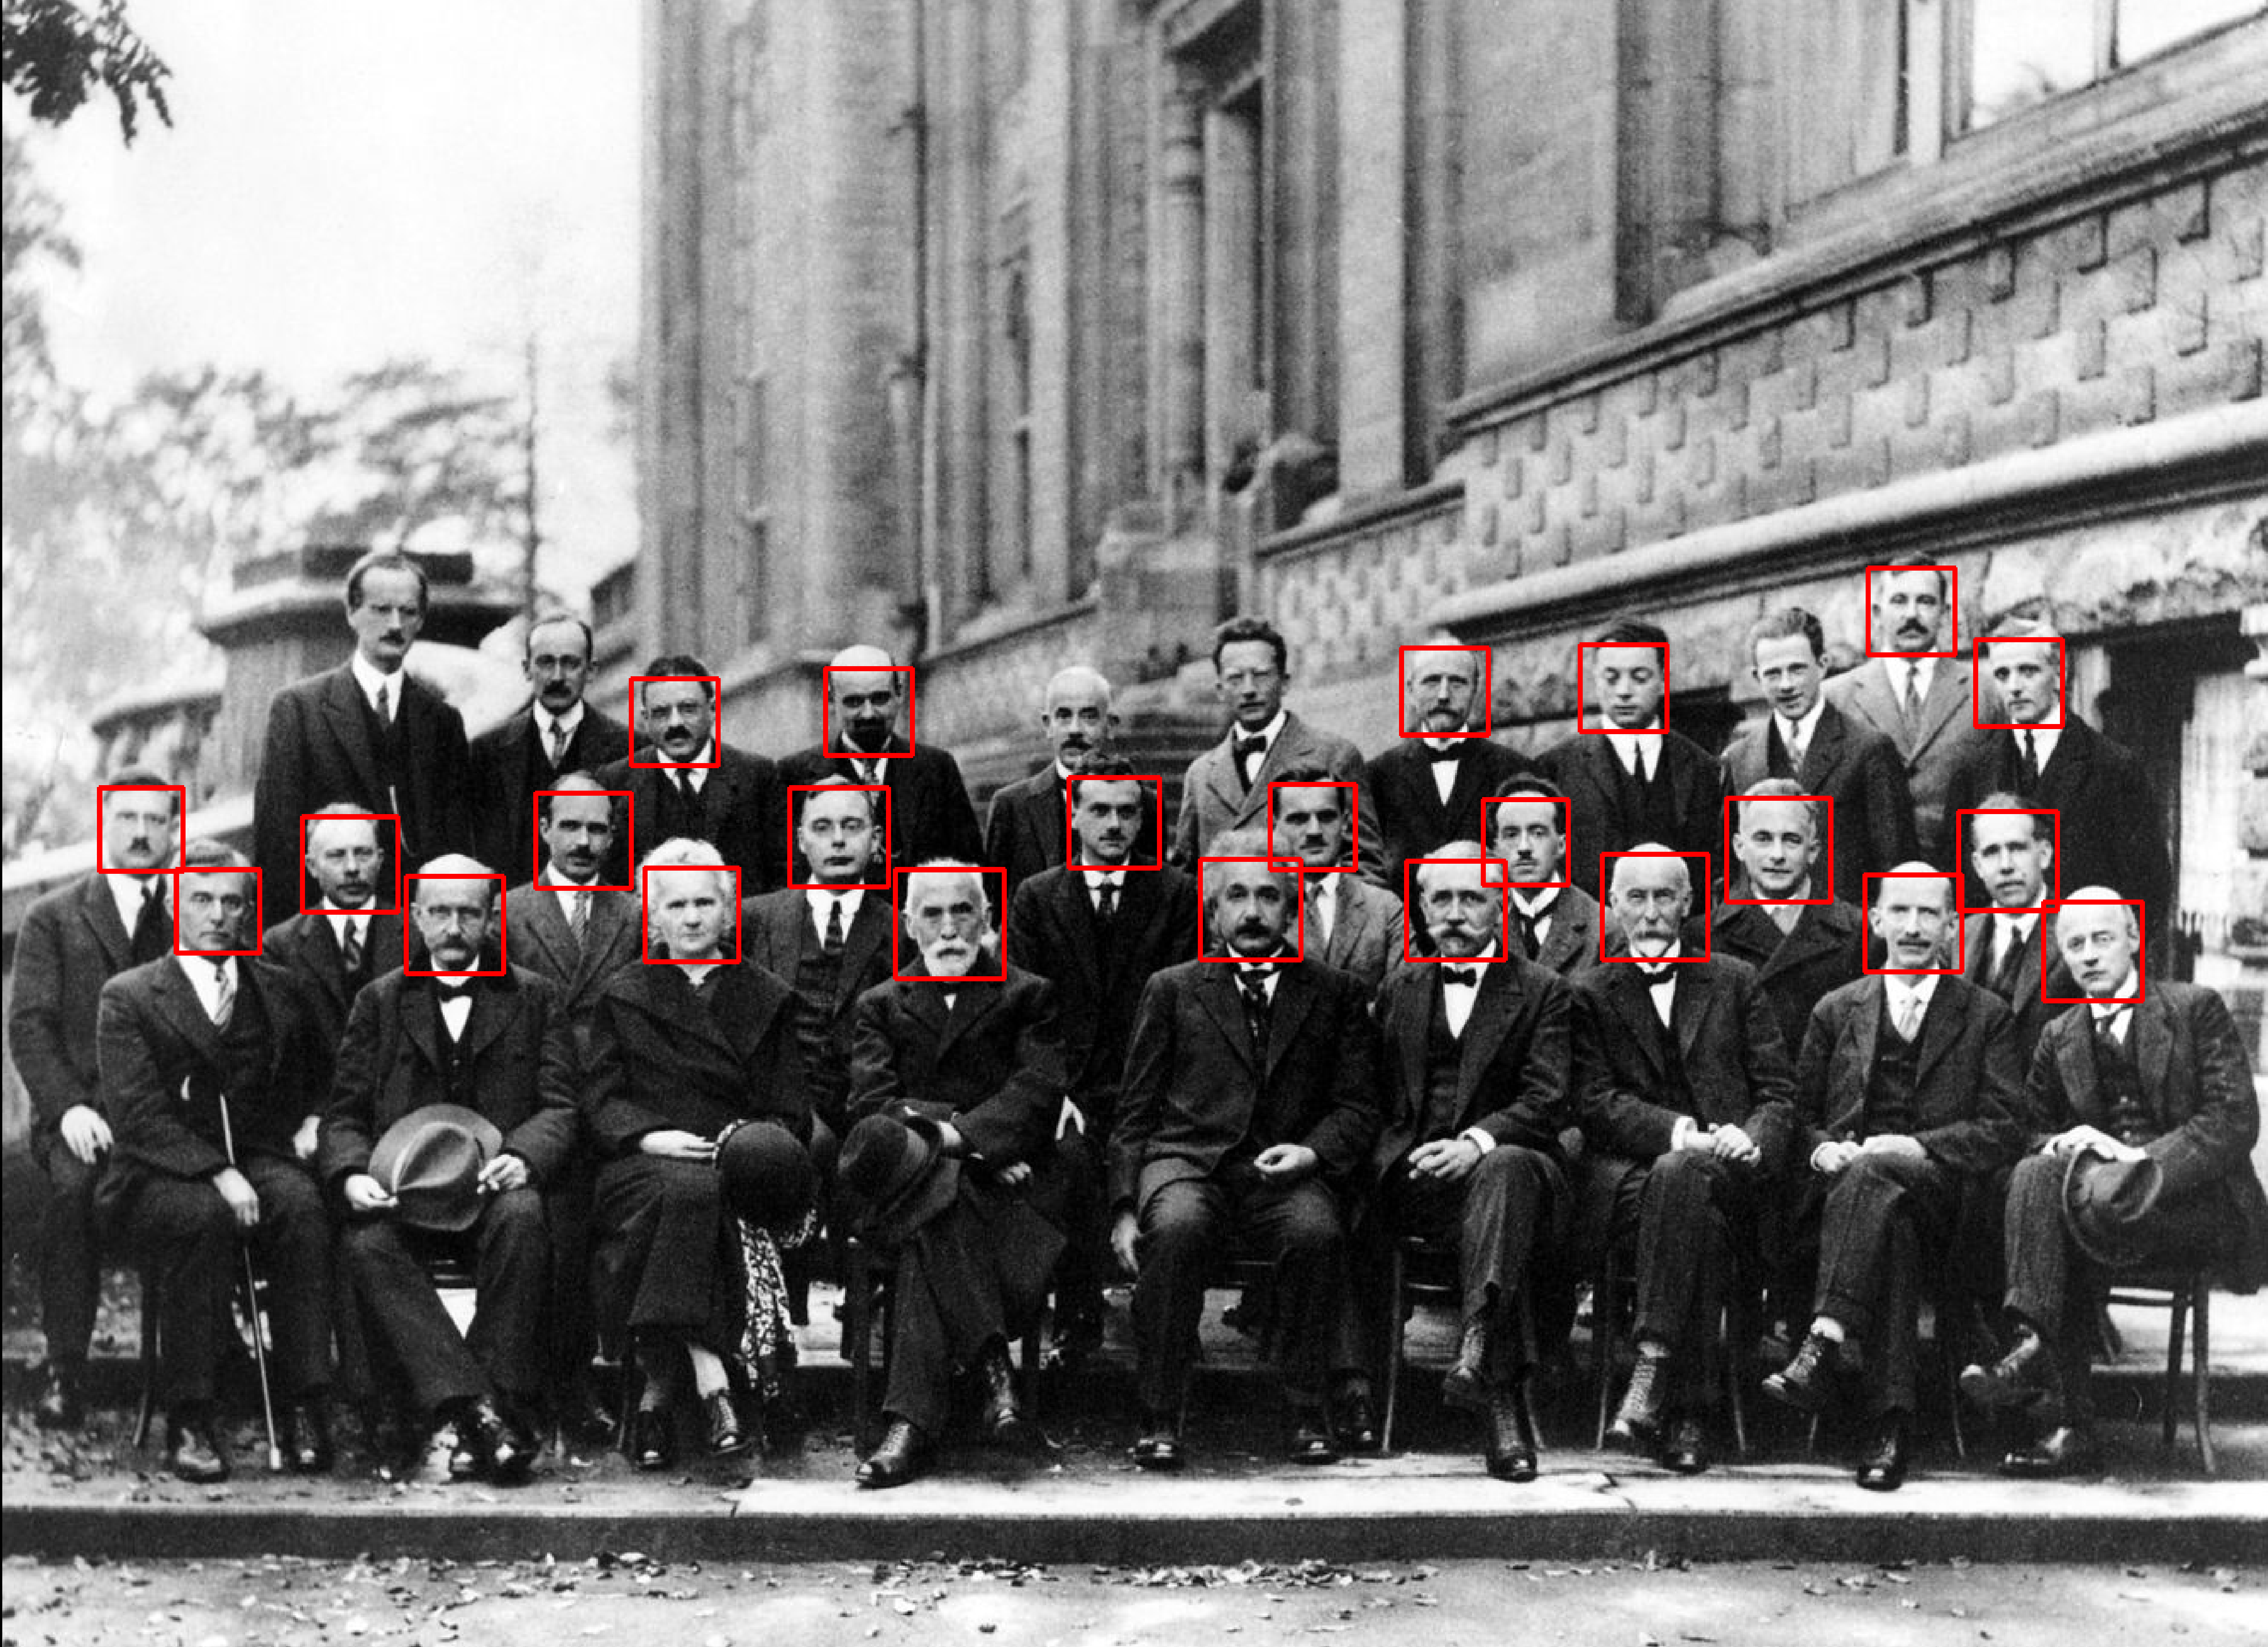
\includegraphics[width=7.5cm]{./figures/har1.png}
        \caption{Front face classifier with scale factor 1.3}
        \label{pic:har1}
    \end{minipage}
    \qquad
    \begin{minipage}[t]{0.47\textwidth}
        \centering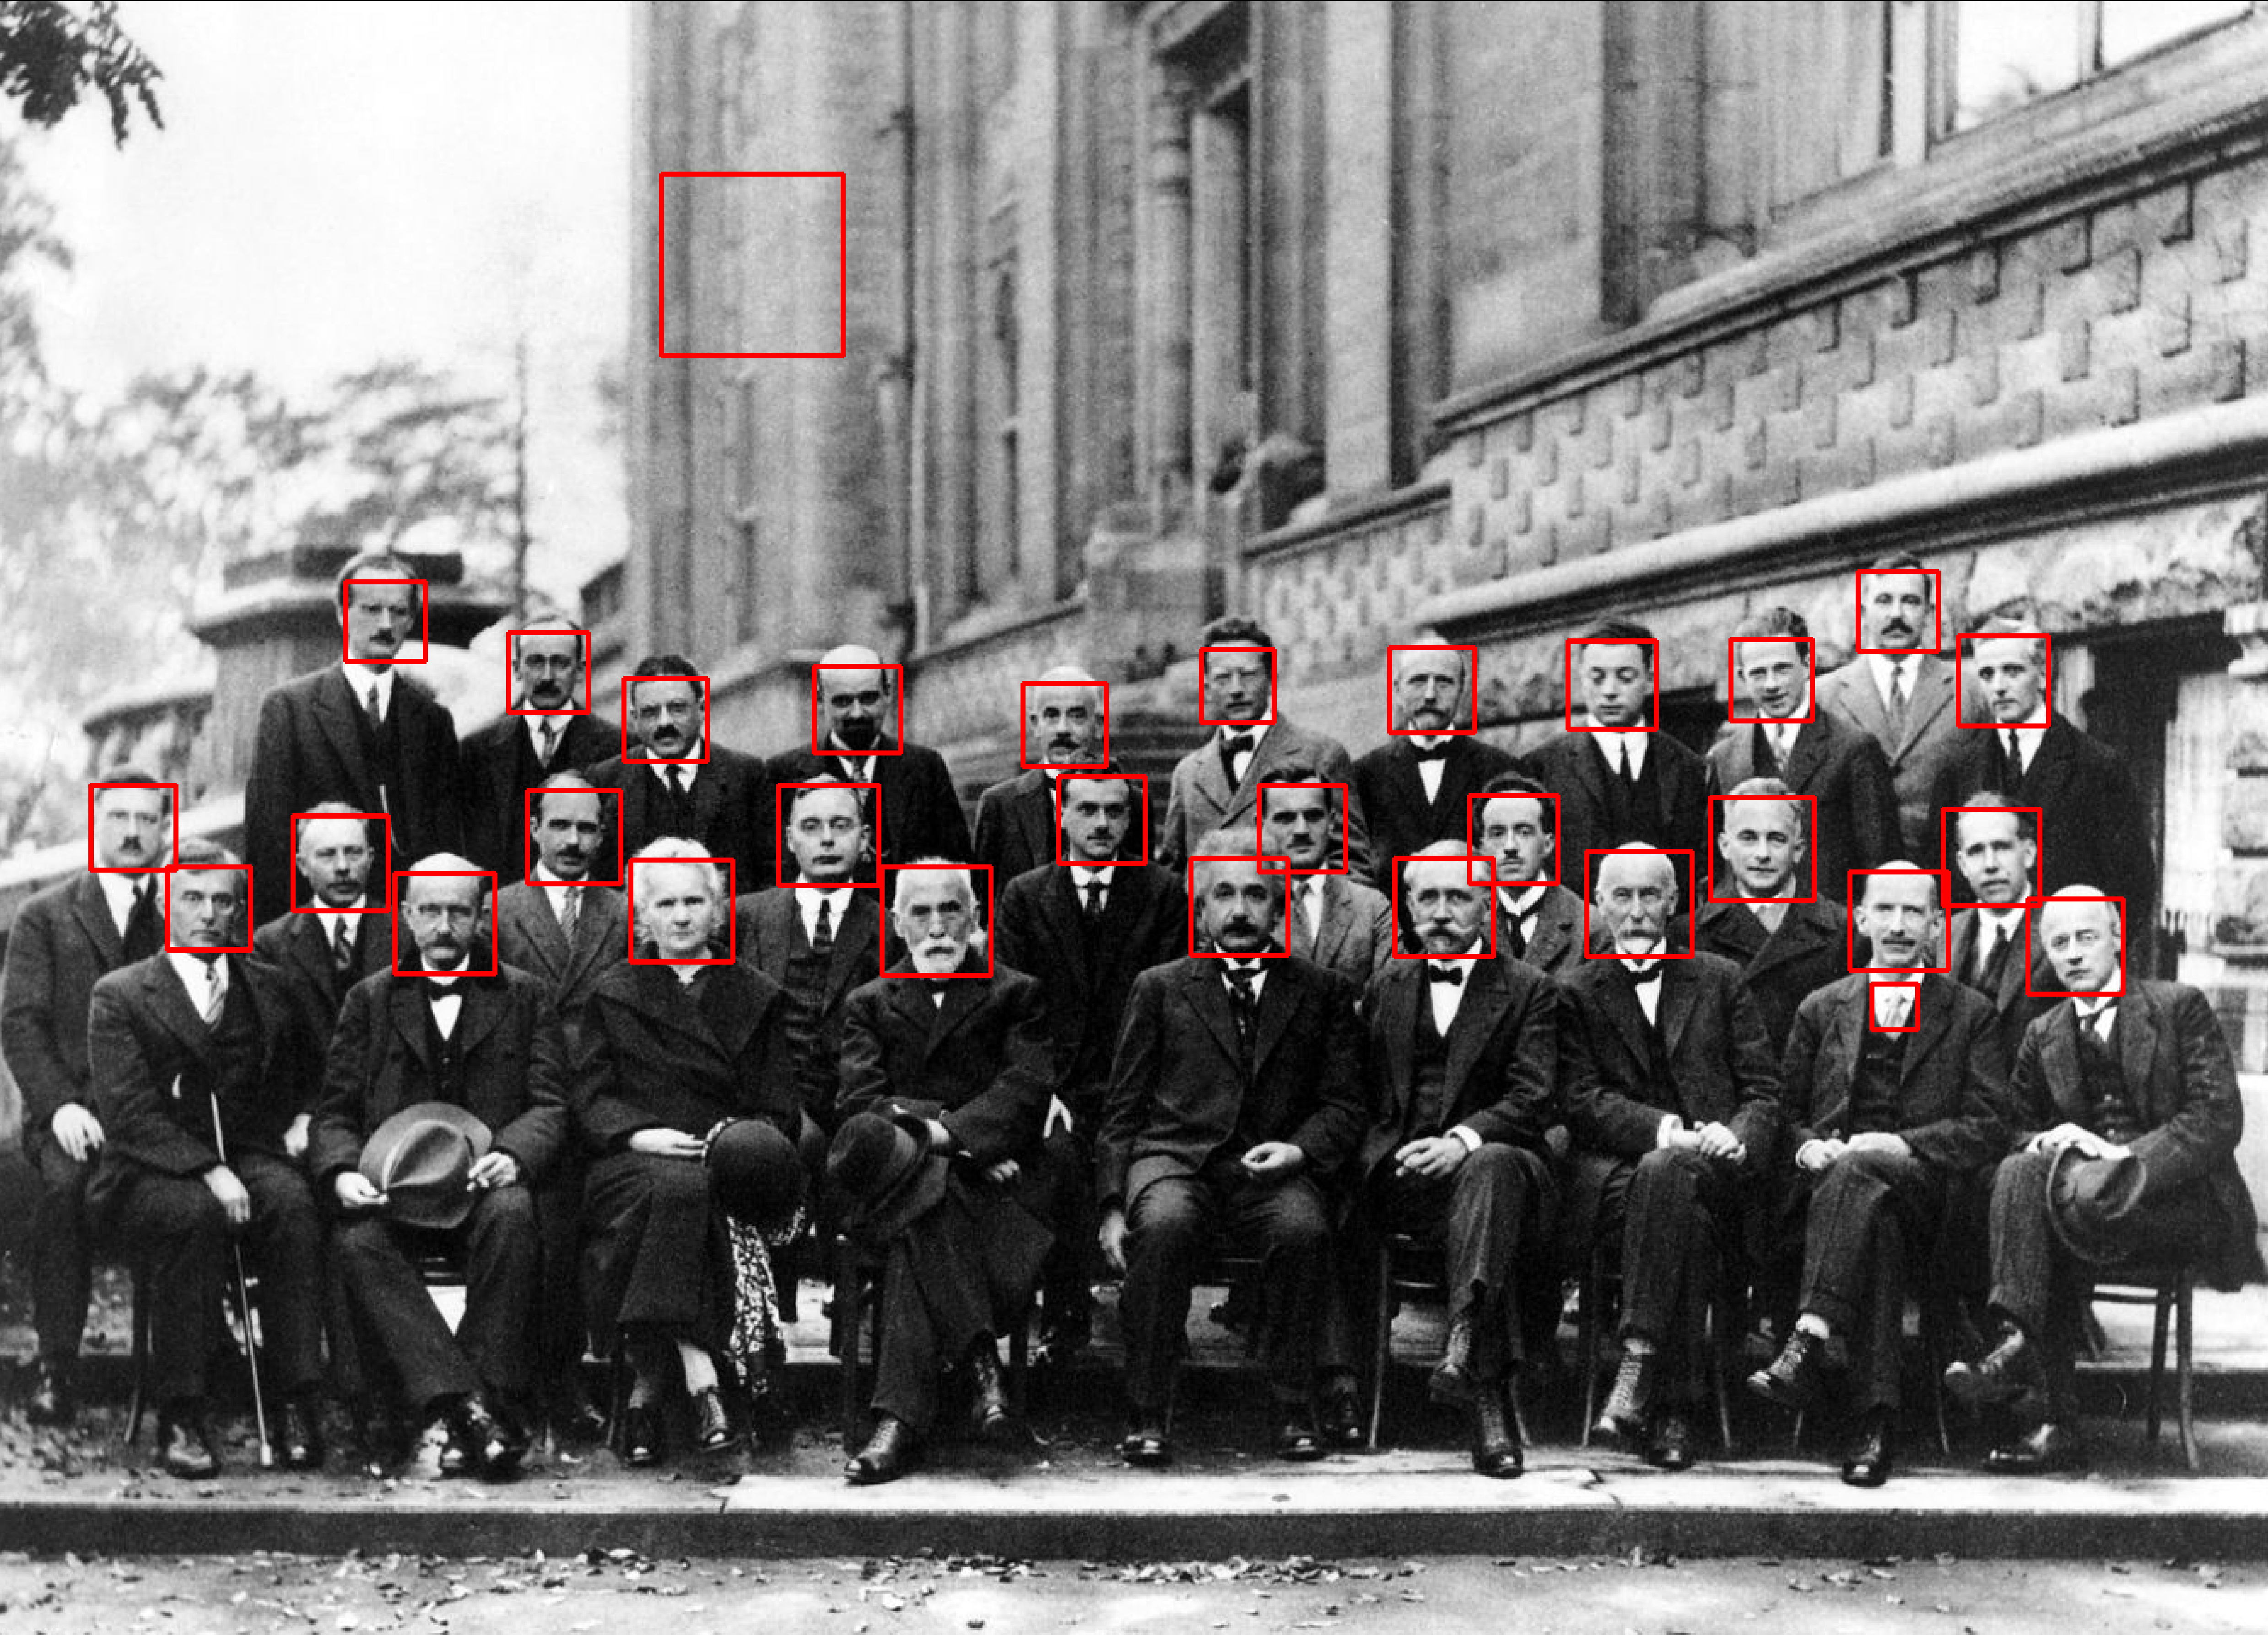
\includegraphics[width=7.5cm]{./figures/har2.png}
        \caption{Front face classifier with scale factor 1.1}
        \label{pic:har2}
    \end{minipage}
\end{figure}
However, detectors of this kind require front faces and standing bodies in order to measure the Haar-like features towards eyes, noses, mouths, ears, faces, etc. The detectors based on Haar-like features may fail when encountering profile faces or faces under complex illuminating conditions. Hence, a scale factor is introduced to struggle for a balance between the false positive and the true negative rate. Fig.\ref{pic:har1} depicts the case when the true negative rate is high while fig.\ref{pic:har2} is the case when the false positive rate is high.

\subsubsection{Multi-task Cascaded Convolutional Networks}
Another advanced face detection tool published in 2017 is the Multi-task Cascaded Convolutional Networks (MTCNN). MTCNN proposes three sub-convolutional neural networks, namely, the proposal network (P-Net), the refine network (R-Net), and the output network (O-Net) to increase the accuracy of detection step by step \cite{xiang2017joint}.   
\begin{figure}[!htbp]
    \centering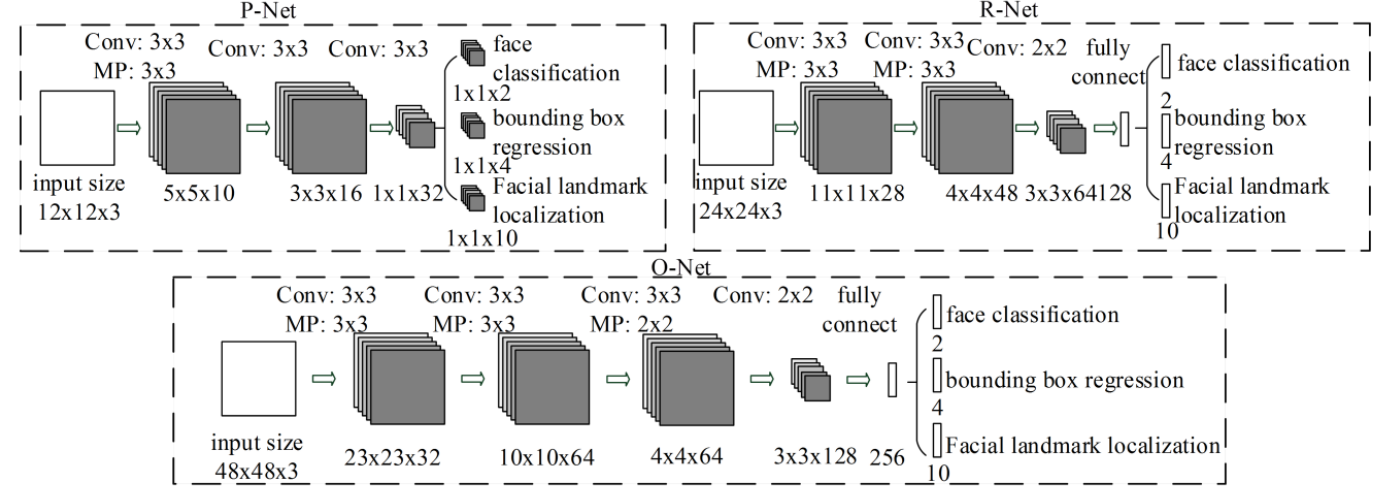
\includegraphics[width=15cm]{./figures/mtcnn1.png}
    \caption{The architectures of P-Net, R-Net, and O-Net, where ``MP'' means max pooling and ``Conv'' means convolution. The step size in convolution and pooling is 1 and 2, respectively.}
    \label{pic:mtcnn1}
\end{figure}

\subsection{Face Recognition}
Once detecting the location of faces, machines try to remember the image patterns by extracting useful features from the faces and then give predictions on new images. We introduce the traditional convolutional neural networks as well as the powerful FaceNet proposed in recent years.


\subsubsection{Feature Extraction}
\paragraph{Convolutional Neural Networks}
The first choice to do the feature extraction is to build convolutional neural networks (CNN). Convolutional layers are adapted to detect the edges and boundaries of faces by performing convolutions or cross-correlations through filters via a moving window approach. Strides and padding can be adjusted to control the shape of the output. The pooling layer then reduces the dimension of the convoluted result by taking the maximum or average of the entries. Fully-connected layers are used to flatten the output tensor into a long vector
to feed into a multi-layer perceptron for final classification purposes.

\paragraph{FaceNet}
FaceNet \cite{schroff2015facenet} is an advanced system proposed by Google that directly learns a mapping from face images to a compact Euclidean space where distances
directly correspond to a measure of face similarity. Fig.\ref{pic:facenet1} and fig.\ref{pic:facenet2} illustrates the facenet model structure and the definition of its target which is to minimize a triplet loss. 
\begin{figure}[H]
    \begin{minipage}[t]{0.47\textwidth}
        \centering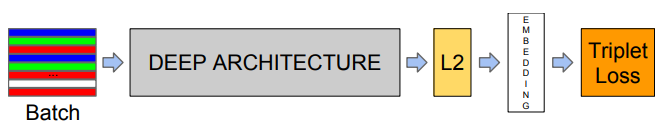
\includegraphics[width=7.5cm]{./figures/facenet1.png}
        \caption{A General model structure for FaceNet consists of a batch input layer and a deep CNN followed by L2 normalization, which results in the face embedding. This is followed by the triplet loss during training.}
        \label{pic:facenet1}
    \end{minipage}
    \qquad
    \begin{minipage}[t]{0.47\textwidth}
        \centering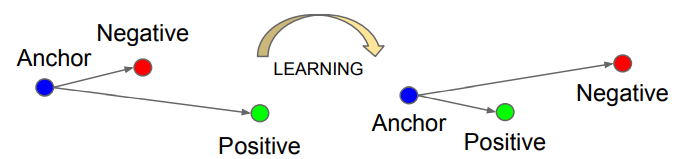
\includegraphics[width=7.5cm]{./figures/facenet2.png}
        \caption{The Triplet Loss minimizes the distance between an anchor and a positive, both of which have the same identity, and maximizes the distance between the anchor and a negative of a different identity.}
        \label{pic:facenet2}
    \end{minipage}
\end{figure}

A detailed model structure is given by fig.\ref{pic:facenetX}, which uses a rather complicated model structure with stochastic gradient descent and standard backpropagation. To avoid overfitting, the model uses AdaGrad to approach the optimal solution slowly, and the results show that the loss decreases drastically after a total training of 500 hours, with a total of roughly 1000 hours. 
\begin{figure}[H]
    \centering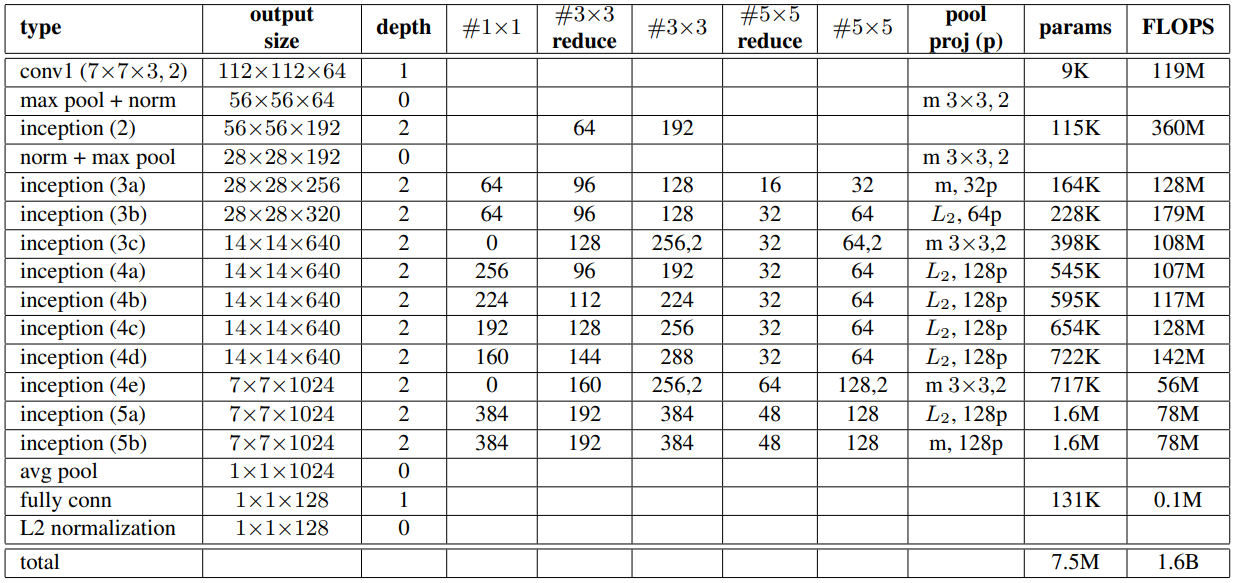
\includegraphics[width=14cm]{./figures/facenetX.png}
    \caption{Network architecture of FaceNet with inception incarnation}
    \label{pic:facenetX}
\end{figure}


\subsubsection{Classifiers}
Traditional face recognition competitions are dominated by support vector machines (SVM). Competition winners conduct feature extraction and use SVM, which successfully maps the features of images to higher or even infinite dimensions (such as the radial kernel) to label the name of a given image. In the deep learning stage, multi-layer perceptrons (MLP) are able to handle complex pattern recognition which is challenging to display and describe. For convolutional neural networks, there has already been an MLP after the fully connected layer to produce the final output. For FaceNet, we can apply either SVM or MLP to receive the inputted features and then produce the classification outcome.

\section{Materials and Methods}
In this project, we try to solve a multi-class celebrity classification problem to answer ``who is this person'' by extracting features from images of celebrities, building different models using the training dataset, and then comparing their performance on the test dataset.

\subsection{Data Description}
We pick a part of (more than 1000 observations) the Bollywood celebrity faces data from Kaggle (\href{https://www.kaggle.com/datasets/havingfun/100-bollywood-celebrity-faces}{100-bollywood-celebrity-faces}) for face recognition purposes. The raw data contains images of different sizes for 13 different Bollywood celebrities. Most images are in jpg format and contain only one front face each. However, some pictures are in other formats, pictures containing more than one face or pictures under complex illuminating conditions. There are generally more than 100 pictures for each celebrity. 


\subsection{Data Preprocessing}

\subsubsection{Train-Test Split}
We randomly split the images for each celebrity into 70\% of training and 30\% of testing. The detailed number for each celebrity is in fig.\ref{pic:train_test}. 
\begin{figure}[!htbp]
    \centering\includegraphics[width=12cm]{./figures/train_test.png}
    \caption{Train-test images distribution}
    \label{pic:train_test}
\end{figure}
However, it should be mentioned that some pictures are of bad quality or even have already been destroyed so that they cannot be used in model fitting or predicting. Hence, the actual number of images participated in the training and testing may be slightly lower than the actual amount.


\subsubsection{Image Processing}
Different face recognition models may pose different requirements for the input formats. These requirements typically include some of the following items:
\begin{itemize}
    \item min-max scaling of pixels for each channel
    \item color conversion (such as BGR to RGB or BGR to grayscale)
    \item standardization of pixels for all channels
    \item image resizing to a given input format
    \item possible face alignment (such as tight crop around the face area)
\end{itemize}
Specifically, almost all the models used for recognition need scaling of the pixels to control the values in the range from 0 to 1. To detect the location of faces, Haar cascaded classifier requires converting the colored picture to grayscale. To successfully extract the features from faces,  CNN and MLP that conduct the feature extraction need to convert the image from BGR to RGB format. MTCNN also needs to convert the image to RGB format, even if the inputted image is grayscale. Some typical pre-trained FaceNet models require that the inputted pixels of pictures are standardized among all the three channels and the inputted size of each channel should be $160\times 160$. MTCNN requires the inputted size of each channel to be $12\times 12$, $24\times 24$, $48\times 48$ for P-Net, R-Net and O-Net. Other models may have different requirements for the inputted size. Details about sizing requirements will be re-emphasized once they appear in the model construction process. 

\subsubsection{One-Hot Encoding}
The recognition problem involves a 13-class classification. Hence we need to perform encoding for the model output. Since direct label encoding may imply the MLP that certain order exists among the category values, we perform one-hot encoding on the output labels to avoid such misleading information and avoid possible overfitting.

\subsection{Models Used}
In the following section, we will first detect the faces from each image using the MTCNN architecture. After obtaining the cropped faces, we will first extract features and conduct classification using self-built CNNs as baseline models. Then we may apply more advanced FaceNet and other renowned models for image classification to compare their performance. For FaceNet, both SVM and MLP will be tested for final classification. Parameters will be tuned and compared in this process. Finally, we will compare the performance and propose some further improvements.

\section{Model Construction and Results}
\subsection{Face Detection with MTCNN}

The advanced face detection model Multi-task Cascaded Convolutional Networks (MTCNN) \cite{xiang2017joint} was published in 2017.
Before using MTCNN, we need to scale the image to different sizes to generate image pyramids for the three convolutional networks of P-Net, R-Net, and O-Net in the MTCNN as mentioned above. The MTCNN first input the 12×12×3 input to P-Net, which helps us generate some candidate boxes for detecting human faces. After that, R-Net selects from the candidate boxes (of size 24×24×3) generated by the previous P-Net and removes a large number of non-face boxes. Finally, O-Net, whose structure is similar to that of R-Net, outputs five additional face key points based on the obtained face area of R-Net (of size 48×48×3). The five key points here include two eyes, a nose, and two mouth corners. The detailed architectures of P-Net, R-Net, and O-Net are as shown in fig.\ref{pic:mtcnn1}. 

For the model training in this section, we use the dataset in ``data\_bw'', where the ``train'' and ``val'' folders correspond to our training and test sets, respectively. Both the training and test sets contain 13 celebrities corresponding to 13 subdirectories. We define the MTCNN detector with default weights and input the processed images to detect faces. And the result of face detection is a list of bounding boxes, where each bounding box ($x, y, w, h$) consists of its lower-left corner coordinates and the width and height of the bounding box. 

For each image in the dataset, we can achieve the purpose of face detection from the bounding box, as shown in fig.\ref{pic:mtcnn2}.
For convenience, we only take the first bounding box from the bounding box list in each image, meaning that there is only one face used in each image. In fact, some pictures contain more than one face of the same star (see fig.\ref{pic:mtcnn3}), but such pictures are rare. Meanwhile, the shooting time and environment of all faces in the same picture are likely to be similar. Hence, the information of the detected faces is also relatively similar, which explains why we can use one of them only without losing much information. 

\begin{figure}[H]
    \begin{minipage}[t]{0.47\textwidth}
        \centering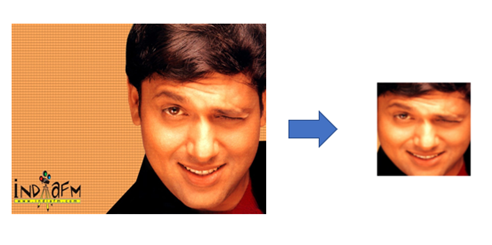
\includegraphics[width=7.5cm]{./figures/mtcnn2.png}
        \caption{Face detection result for\\ image ‘/data\_bw/val/Govinda/12.jpg'}
        \label{pic:mtcnn2}
    \end{minipage}
    \qquad
    \begin{minipage}[t]{0.47\textwidth}
        \centering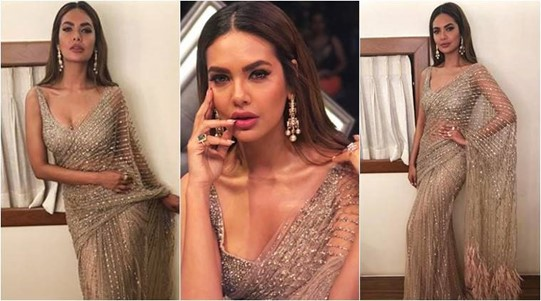
\includegraphics[width=7.5cm]{./figures/mtcnn3.jpg}
        \caption{Image with three faces\\ in ‘data\_bw/train/Esha\_Gupta'}
        \label{pic:mtcnn3}
    \end{minipage}
\end{figure}

Lastly, we save the result as a numpy ``npz'' format file and save it in ``data\_bw.npz''. Some face detection results in the test set of Deepika Padukone are shown in fig.\ref{pic:mtcnn4}. Obviously, each face of Deepika Padukone is correctly detected, and the illumination, skin color, and orientation of the face are diverse.

\begin{figure}[H]
    \centering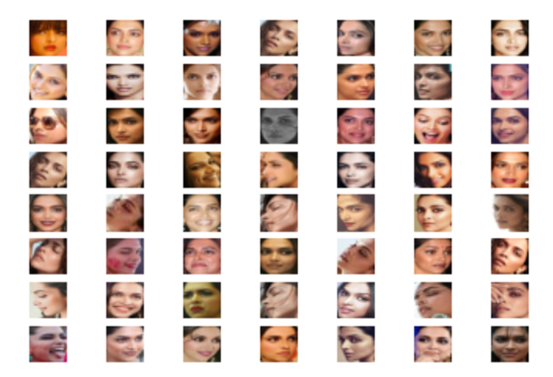
\includegraphics[width=12cm]{./figures/mtcnn4.png}
    \caption{Face detection results for 56 images in ‘data\_bw/val/Deepika\_Padukone/'}
    \label{pic:mtcnn4}
\end{figure}

\subsection{Feature Extraction and Classification}

\subsubsection{Convolutional Neural Networks}
\paragraph{Model 1}
After using MTCNN, the outputted images are of size $160 \times 160 \times 3$ and are in RGB format. We then convert the images into tensors and divide the components by 255 to scale the input. The training tensors are then randomly shuffled and then one-hot encoding is performed on both the training labels and test labels.

We now provide two self-built convolutional neural networks as baseline models. The core structure of the first CNN is summarized in the code below.
\begin{lstlisting}[language=python]
tf.random.set_seed(4012)
# construct the CNN model 1
model = Sequential()
model.add(Conv2D(filters=32,kernel_size=(5,5),padding='same', 
                 activation='relu',input_shape=(160,160,3)))
model.add(Conv2D(filters=32,kernel_size=(5,5),padding='same', 
                 activation='relu'))
model.add(MaxPool2D(pool_size=(2,2)))
model.add(Dropout(0.25))
model.add(Conv2D(filters=64,kernel_size=(3,3),padding = 'same', 
                 activation='relu'))
model.add(Conv2D(filters=64,kernel_size=(3,3),padding='same', 
                 activation='relu'))
model.add(MaxPool2D(pool_size=(2,2),strides=(2,2)))
model.add(Dropout(0.25))
model.add(Flatten())
model.add(Dense(256,activation="relu"))
model.add(Dropout(0.5))
model.add(Dense(13,activation="softmax"))
model.compile(optimizer='adam',loss="binary_crossentropy",metrics=["accuracy"])
model.fit(trainX,trainy,batch_size=64,epochs=50,validation_split=0.2)
# evaluate on the test dataset
model.evaluate(testX,testy)
\end{lstlisting}
\vspace{-0.6cm}
Firstly two convolutional layers with 32 filters are applied to extract the features. Since the output of MTCNN is of size $160\times 160$, we set the inputted size to be the same. The inputted faces are in RGB format and the number of channels is 3. Then we add a maximum pooling layer to reduce the dimension. Similar operations are done for another time but with 64 filters and smaller kernel sizes. The dropout layer is used to drop some of the neurons in a given layer for a probability of 0.25. After extracting features, we add a fully-connected layer to flatten the output into a long vector. A layer of 256 neurons with RELU activation is followed after the flattening layer, with a dropout probability of 0.5 to avoid possible overfitting. Finally, we add an output layer to output the predicted probability for the 13 classes. The predicted outcome will be in a one-hot encoding 2-dimensional array. After fitting on the training dataset, we will evaluate the performance on the test dataset. 

Binary cross-entropy is used for the multi-class classification problem, and it is defined as:
\begin{equation}
    \varepsilon^{(t)} = -\frac{1}{13}\sum_{p=1}^{13}\left[  \tilde{y_p}^{t} \times ln(a_p^{(L,t)}) + (1-\tilde{y_p}^{t}) \times ln(1-a_p^{(L,t)}) \right]
\end{equation}
where for a given label y taking values $c_1,\dots, c_{13}$, $\tilde{y_p}^{t}=1$ if actual label $y=c_p$ and zero otherwise, for $p=1,\dots , 13$. We use a batch size of 64 pictures and use the Adaptive Moment Estimation (Adam) as the activation function, which is also the common choice for many other deep learning tasks. The training images are randomly shuffled and we pick 20\% of them to serve as the validation set.

In a total of 50 epochs, we plot the training accuracy and the validation accuracy in fig.\ref{pic:cnn1}, together with the training and validation loss. 
\begin{figure}[!htbp]
    \centering\includegraphics[width=16cm, height=5cm]{./figures/cnn1.png}
    \caption{Train (Validation) accuracy (loss) changes as number of epochs increases}
    \label{pic:cnn1}
\end{figure}
It can be seen that the training accuracy converges rapidly, but the validation accuracy stays at roughly 50\% after 15 epochs and then keeps fluctuating. The training loss decreases sharply, yet the validation loss first drops and then increases after 15 epochs, indicating a risk of overfitting. There are several possible reasons:
\begin{itemize}
    \item The male bollywood celebrities in the dataset look similar and the faces contain different illuminating conditions with different extents of face masking.
    \item The parameters (most likely the learning rate) is not appropriate.
    \item The model structure is too simple to capture the face characteristics.
\end{itemize}

We now plot some of the correctly and incorrectly identified images. Many corrected labeled images are standard front faces, with seldom face coverings or complex illuminating conditions. However, some of the incorrectly labeled celebrities have hands covering their mouths. Some are showing their profile so that information on one eye will be missing. Some wear dark sunglasses so that the information can be misleading to the machine. 
\begin{figure}[H]
    \begin{minipage}[t]{0.47\textwidth}
        \centering\includegraphics[width=7.2cm]{./figures/correct.png}
        \caption{Correctly identified celebrity images}
        \label{pic:correct1}
    \end{minipage}
    \qquad
    \begin{minipage}[t]{0.47\textwidth}
        \centering\includegraphics[width=7.5cm]{./figures/mislabeled.png}
        \caption{Incorrectly identified celebrity images}
        \label{pic:wrong1}
    \end{minipage}
\end{figure}
These are possible reasons that the CNN gives wrong predictions. However, there are still lots of images of front faces that the machine gives wrong predictions. We summarize the accuracy, weighted average precision and recall rate, and the F1-score of the predicted result on the test dataset.
\begin{table*}[!htbp]
    \small
	\centering
	\begin{tabularx}{0.6\textwidth}{ccccc}
		\toprule
		\textbf{Support}
       &  \textbf{Accuracy}
        & \textbf{Precision} 
        & \textbf{Recall} 
        & \textbf{F1-Score} \\

        \midrule
        452
        & 51\%
        & 49\%
        & 52\%
        & 50\%\\
		\bottomrule
	\end{tabularx}%
	\label{tab:result1}%
	\caption{Performance indicator on the test set}
\end{table*}%

Unfortunately, the self-built CNN only gives a prediction accuracy of 51\% on the test set. We further plot the confusion matrix of the training and test set to look into details.

\begin{figure}[H]
    \begin{minipage}[t]{0.49\textwidth}
        \centering\includegraphics[width=7.5cm]{./figures/cnn1_confusion_train.png}
        \caption{Confusion matrix on the training set}
        \label{pic:confusion1}
    \end{minipage}
    \qquad
    \begin{minipage}[t]{0.49\textwidth}
        \centering\includegraphics[width=7.2cm]{./figures/cnn1_confusion2.png}
        \caption{Confusion matrix on the test set}
        \label{pic:confusion2}
    \end{minipage}
\end{figure}
The model achieves a pretty high accuracy on the training dataset after 20 epochs despite some errors made in predicting Disha Patani. However, the model fails to generalize in the test set. For Bobby Deol, the CNN predicts his images as all kinds of other stars. We now seek to improve the model with more tricks on the layers and parameters. 

\paragraph{Model 2}
After more trials and tunings with the layers and model parameters, we now improve the model structure to the following.

\begin{lstlisting}[language=python]
tf.random.set_seed(4012)
# add call-back mechanism
learning_rate_reduction = ReduceLROnPlateau(monitor='val_accuracy', 
                      patience=3, 
                      verbose=1, 
                      factor=0.7, 
                      min_lr=0.00000000001)
# construct the CNN model 2
model = Sequential()
model.add(Conv2D(filters=20,kernel_size=(5,5),padding='Same', 
                 activation='relu',input_shape=(160,160,3)))
model.add(MaxPool2D(pool_size=(2,2)))
model.add(Dropout(0.25))
model.add(Conv2D(filters=50,kernel_size=(6,6),padding='Same', 
                 activation='relu'))
model.add(MaxPool2D(pool_size=(2,2)))
model.add(Dropout(0.25))
model.add(Conv2D(filters=150,kernel_size=(5,5),padding='Same', 
                 activation='relu',input_shape=(160,160,3)))
model.add(Flatten())
model.add(Dense(256, activation="relu"))
model.add(BatchNormalization())
model.add(Dropout(0.5))
model.add(Dense(13,activation="softmax"))
model.compile(optimizer='adam',loss="binary_crossentropy",metrics=["accuracy"])
history = model.fit(trainX,trainy,batch_size=32,epochs=50,validation_split=0.2, callbacks=[learning_rate_reduction])
# evaluate on the test dataset
model.evaluate(testX,testy)
\end{lstlisting}
\vspace{-0.6cm}
Instead of blindly adding convolutional and dense layers, we adopt three convolutional layers but with an increasing number of filters. We also adopt dropout layers to accelerate the training as well as avoid overfitting. We add a batch normalization layer and a dropout layer for the dense layer to accelerate the training further and prevent the vanishing gradient problem. More importantly, we add a callback mechanism. As mentioned previously, the training accuracy improves fast while the validation set increases slowly. This indicates the learning rate is difficult to control even if we use Adam to adjust the learning rate as the number of epoches increases. A callback mechanism reduces the learning rate when a metric stops improving. Here we set the monitor to be the validation accuracy. If the validation accuracy does not increase for 3 epochs (denoted as the ``patience'' parameter), then the learning rate will be reset as 70\% of the previous learning rate (denoted as the ``factor'' parameter). 

We now plot the training accuracy and the validation accuracy, together with the training and validation loss. 
\begin{figure}[!htbp]
    \centering\includegraphics[width=16cm, height=5cm]{./figures/cnn2.png}
    \caption{Train (Validation) accuracy (loss) changes as number of epochs increases}
    \label{pic:cnn2}
\end{figure}
It is easily seen that the model with a callback mechanism performs much better than the previous one. The accuracy now rises up to 60\% roughly and stabilizes after 50 epochs. The validation loss does not fluctuate that much and it slowly stabilizes to 0.2. 
\begin{figure}[H]
    \begin{minipage}[t]{0.47\textwidth}
        \centering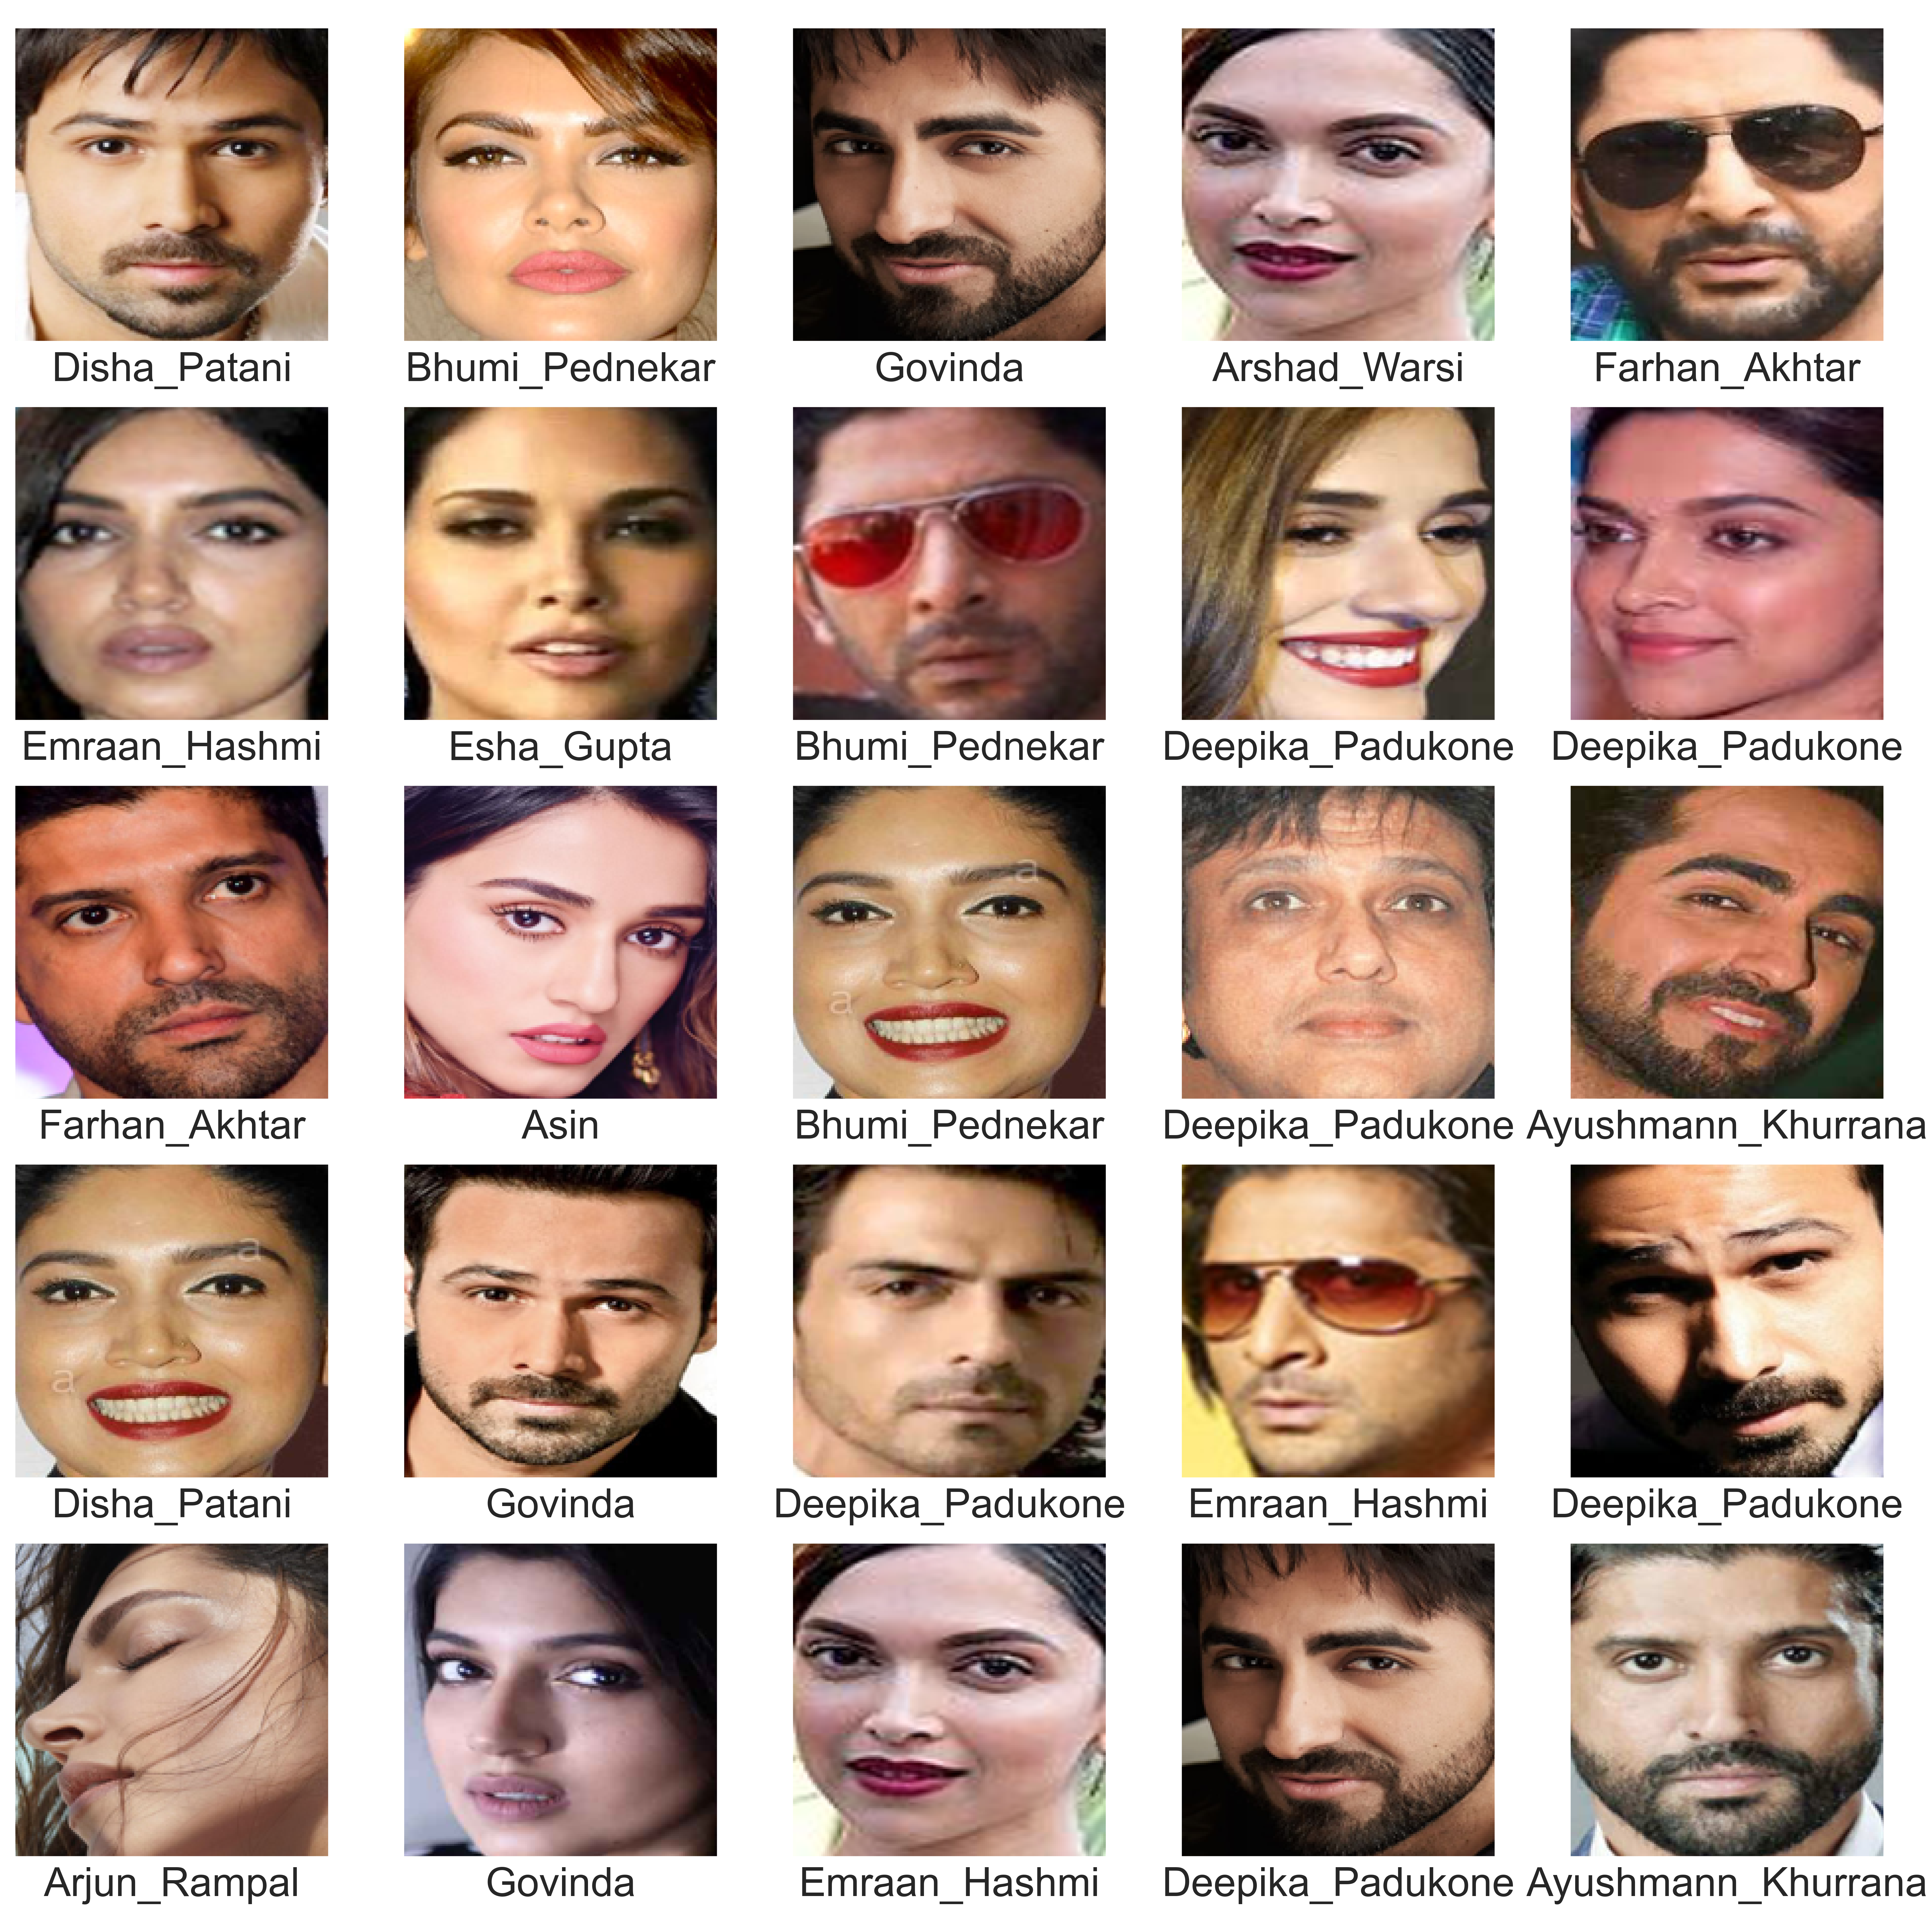
\includegraphics[width=7.5cm]{./figures/correct2.png}
        \caption{Correctly identified celebrity images}
        \label{pic:correct2}
    \end{minipage}
    \qquad
    \begin{minipage}[t]{0.47\textwidth}
        \centering\includegraphics[width=7.5cm]{./figures/mislabeled2.png}
        \caption{Incorrectly identified celebrity images}
        \label{pic:wrong2}
    \end{minipage}
\end{figure}
This indicates the callback mechanism proves useful in controlling the learning rate and stabilizes the performance on the validation set. We again plot some of the correctly and incorrectly predicted images. Obviously, some of the incorrectly labeled images are under rather complicated illuminating conditions. Some celebrities make faces so that their mouths are open and eyes are closed. Some images are so dark that it is almost impossible to recognize even directly by our eyes. 
\begin{table*}[!htbp]
    \small
	\centering
	\begin{tabularx}{0.6\textwidth}{ccccc}
		\toprule
		\textbf{Support}
       &  \textbf{Accuracy}
        & \textbf{Precision} 
        & \textbf{Recall} 
        & \textbf{F1-Score} \\

        \midrule
        452
        & 60\%
        & 65\%
        & 57\%
        & 59\%\\
		\bottomrule
	\end{tabularx}%
	\label{tab:result2}%
	\caption{Performance indicator on the test set}
\end{table*}%
We now summarize the performance metrics of the improved model. The test accuracy now reaches 60\% and the weighted average precision reaches 65\%. The confusion matrix on the training set and test set is shown in fig.\ref{pic:confusion3} and fig.\ref{pic:confusion4}. 
\begin{figure}[H]
    \begin{minipage}[t]{0.49\textwidth}
        \centering\includegraphics[width=7.2cm]{./figures/cnn2_confusion_train.png}
        \caption{Confusion matrix on the training set}
        \label{pic:confusion3}
    \end{minipage}
    \qquad
    \begin{minipage}[t]{0.49\textwidth}
        \centering\includegraphics[width=7.2cm]{./figures/cnn2_confusion.png}
        \caption{Confusion matrix on the test set}
        \label{pic:confusion4}
    \end{minipage}
\end{figure}
Although the improved CNN model still performs unsatisfactorily in predicting images for Bobby Deol, the overall precision and recall all increase compared to the previous one. However, the self-built CNN fails to give a promising prediction result, namely, over 80\% on the test set. The training dataset is still small in number. We need to seek more advanced image recognition model structures proposed in the literature or classifiers designated to solve face recognition problems such as FaceNet to help with the classification.


\subsubsection{Classical CNN Architectures}

Transfer learning is popular to improve the performance when the training data is not enough. It refers to an idea that neural networks trained for one task may be applied to another task and still get a relatively good performance even though the training data is not enough. Many low-level features, such as edge detection and curves detection, can be learned based on a very large data set previously and can then be applied and modified for specific usages. This section will use various pre-trained image recognition models in computer vision and do some fine-tuning modifications for this celebrity face recognition task to compare the performance.

\paragraph{AlexNet Architecture}

 AlexNet CNN architecture\cite{krizhevsky2012imagenet} was proposed by Alex Krizhevsky, Ilya Sutskever and Geoffery Hinton in 2012 and it won the Imagenet large-scale visual recognition challenge that year. In this competition, AlexNet showed that deep convolutional neural network can be used for solving image classification problems. The architecture was larger and deeper compared to Lenet-5, and it was the first CNN architecture that stacked convolutional layers directly on top of one another. 

\begin{figure}[H]
    \centering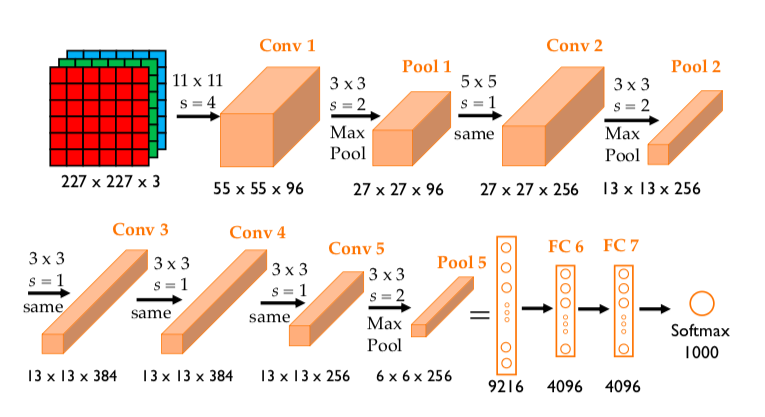
\includegraphics[width=12cm]{./figures/alexnet1.png}
    \caption{AlexNet-Architecture}
    \label{pic:alexnet}
\end{figure}

 This CNN architecture contains eight layers with learnable parameters. The first five layers are convolutional layers followed by max pooling layers, and the remaining three are fully-connected layers. The chosen activation function was ReLU, which is commonly used in CNN fitting.
 
\begin{lstlisting}[language=python]
# AlexNet
model = keras.models.Sequential([
    keras.layers.Conv2D(filters=96, kernel_size=(11,11), strides=(4,4), activation='relu', input_shape=(160,160,3)),
    keras.layers.BatchNormalization(),
    keras.layers.MaxPool2D(pool_size=(3,3), strides=(2,2)),
    keras.layers.Conv2D(filters=256, kernel_size=(5,5), strides=(1,1), activation='relu', padding="same"),
    keras.layers.BatchNormalization(),
    keras.layers.MaxPool2D(pool_size=(3,3), strides=(2,2)),
    keras.layers.Conv2D(filters=384, kernel_size=(3,3), strides=(1,1), activation='relu', padding="same"),
    keras.layers.BatchNormalization(),
    keras.layers.Conv2D(filters=384, kernel_size=(3,3), strides=(1,1), activation='relu', padding="same"),
    keras.layers.BatchNormalization(),
    keras.layers.Conv2D(filters=256, kernel_size=(3,3), strides=(1,1), activation='relu', padding="same"),
    keras.layers.BatchNormalization(),
    keras.layers.MaxPool2D(pool_size=(3,3), strides=(2,2)),
    keras.layers.Flatten(),
    keras.layers.Dense(4096, activation='relu'),
    keras.layers.Dropout(0.5),
    keras.layers.Dense(4096, activation='relu'),
    keras.layers.Dropout(0.5),
    keras.layers.Dense(13, activation='softmax')
])
model.compile(loss='sparse_categorical_crossentropy', optimizer=tf.optimizers.SGD(lr=0.001), metrics=['accuracy'])
history = model.fit(train_ds,epochs=50,validation_data=validation_ds,validation_freq=1,callbacks=[tensorboard_cb])

\end{lstlisting}
\vspace{-0.6cm}

In practice, we not only built our model based on standardized AlexNet structure, but also tried to replace the loss function "sparse categorical crossentropy" by "binary crossentropy" and replace the optimizer "SGD" by "Adam", which is just similar with our model1. However, the predicted result was not improved. What's more, to apply the sparse categorical crossentropy, we need to shuffle and batch the dataset before training. And AlexNet take input image size 227x227, which requires us to resize the imput image.

In the training procedure, the total number of epochs is 50, and the summary of accuracy plot is showed below. It can be observed that the training accuracy converges gradually, and the validation accuracy converges to roughly 62\% after 20 epochs.


\begin{figure}[H]
    \centering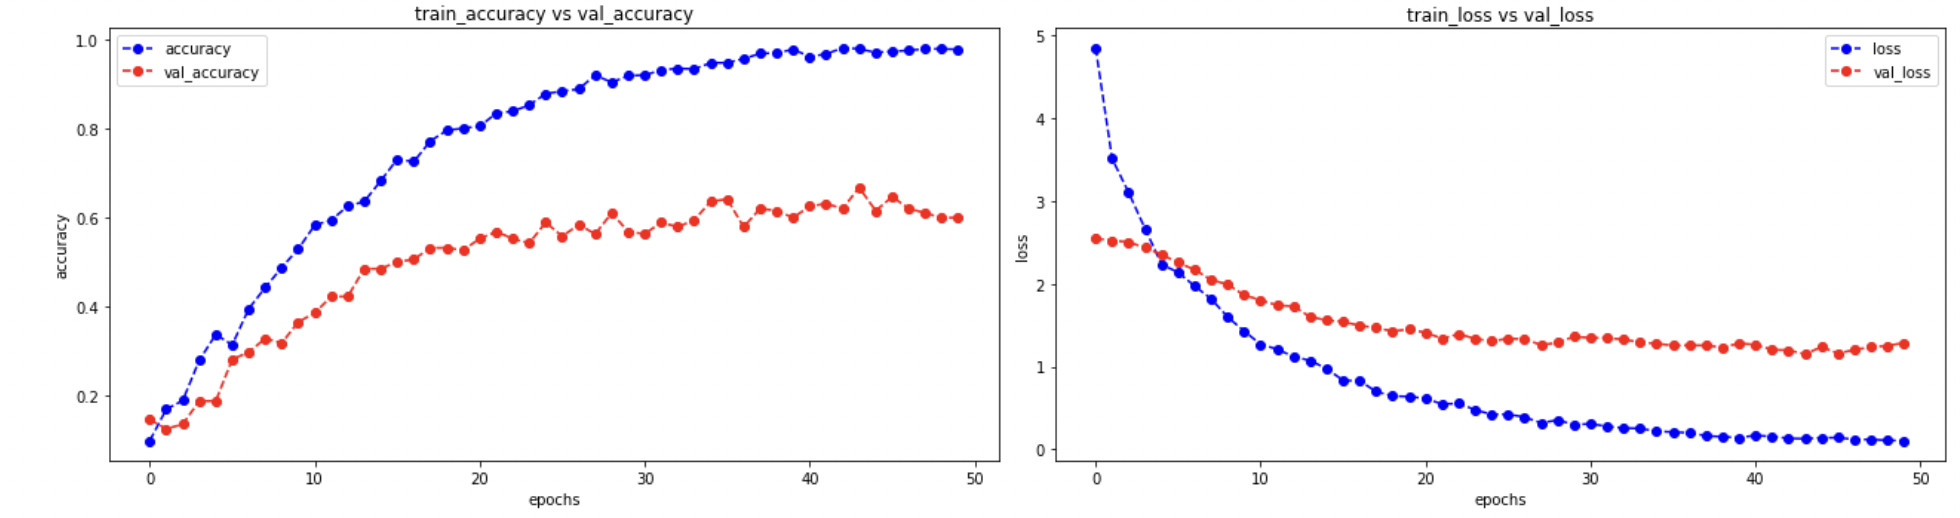
\includegraphics[width=16cm, height=5cm]{./figures/Alexnet2.jpg}
    \caption{Train (Validation) accuracy (loss) changes as number of epochs increases}
    \label{pic:loss-Alexnet}
\end{figure}

The accuracy, weighted average precision, recall rate and F1-score of the predicted result is stated below. It is slightly improved in comparison with model1, yet still not so accurate. Thus, we will consider more CNN architectures that are raised more recently and more complex.



\begin{table*}[!htbp]
    \small
	\centering
	\begin{tabularx}{0.6\textwidth}{ccccc}
		\toprule
		\textbf{Support}
       &  \textbf{Accuracy}
        & \textbf{Precision} 
        & \textbf{Recall} 
        & \textbf{F1-Score} \\

        \midrule
        452
        & 62\%
        & 63\%
        & 62\%
        & 62\%\\
		\bottomrule
	\end{tabularx}%
	\label{tab:result6}%
	\caption{Performance indicator on the test set}
\end{table*}%



\paragraph{VGG16 Architecture}

 VGG16\cite{simonyan2014very} was proposed by Karen Simonyan and Andrew Zisserman of the Visual Geometry Group Lab of Oxford University in 2014. This model won the 1st  and 2nd place on the 2014 ILSVRC challenge. Fig 24. shows the architecture of VGG16:
 
\begin{figure}[H]
    \centering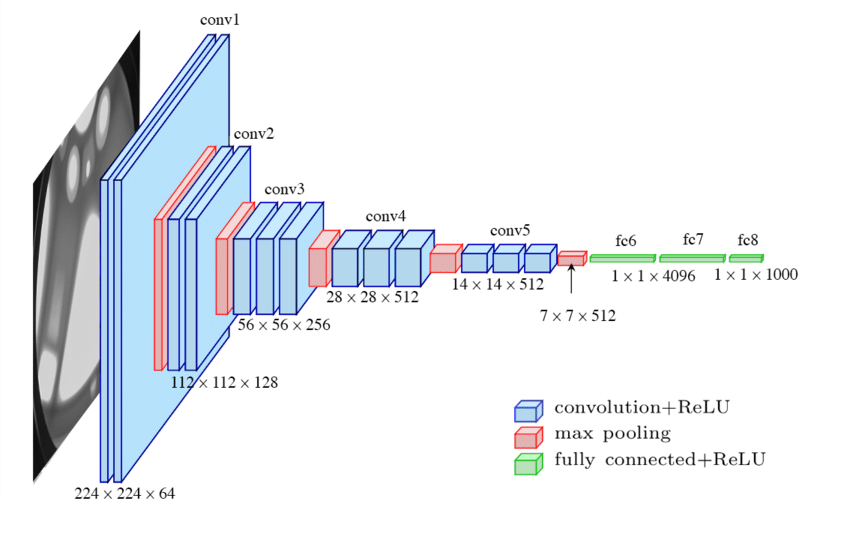
\includegraphics[width=12cm]{./figures/VGG16.png}
    \caption{VGG16-Architecture}
    \label{pic:vgg16}
\end{figure}

In these convolution and pooling layers, the filters used are of the size $3\times 3$ instead of $11\times 11$ in the AlexNet. For some of the layers, a $1\times 1$ pixel is used to manipulate the number of input channels. There is a padding of the 1-pixel (same padding) after each convolution layer to prevent the spatial feature of the image.

After the stack of convolution and max-pooling layer, we flatten this output based on the pre-trained model to make it a 1-d feature vector with length 32768. After this, 3 fully connected layers are fine-tuned by ourselves.

\begin{lstlisting}[language=python]
from keras.applications.vgg16 import VGG16
from keras.applications.vgg16 import preprocess_input
from keras.models import Model
vgg = VGG16(include_top=False, weights='imagenet', input_shape=(160,160,3))
for layer in vgg.layers:
    layer.trainable=False
x = Flatten()(vgg.output)
x = Dense(512,activation='relu')(x)
x = Dense(256,activation='relu')(x)
x = Dense(128,activation='relu')(x)
prediction = Dense(13,activation='softmax')(x)
model = Model(inputs=vgg.input, outputs=prediction)
model.compile(optimizer='adam', loss='categorical_crossentropy', metrics=['accuracy'],weighted_metrics=[tf.keras.metrics.Precision(), tf.keras.metrics.Recall()])
history=model.fit_generator(train_data,validation_data=test_data,epochs=20,steps_per_epoch=len(train_data),alidation_steps=len(test_data))
\end{lstlisting}
\vspace{-0.6cm}

In a total of 20 epochs, we plot the training accuracy and the validation accuracy in fig.\ref{pic:loss-vgg16}, together with the training and validation loss. It can be seen that the training accuracy converges rapidly to 1, the validation accuracy stays at roughly 80\% after 8 epochs and then keeps fluctuating.

\begin{figure}[H]
    \centering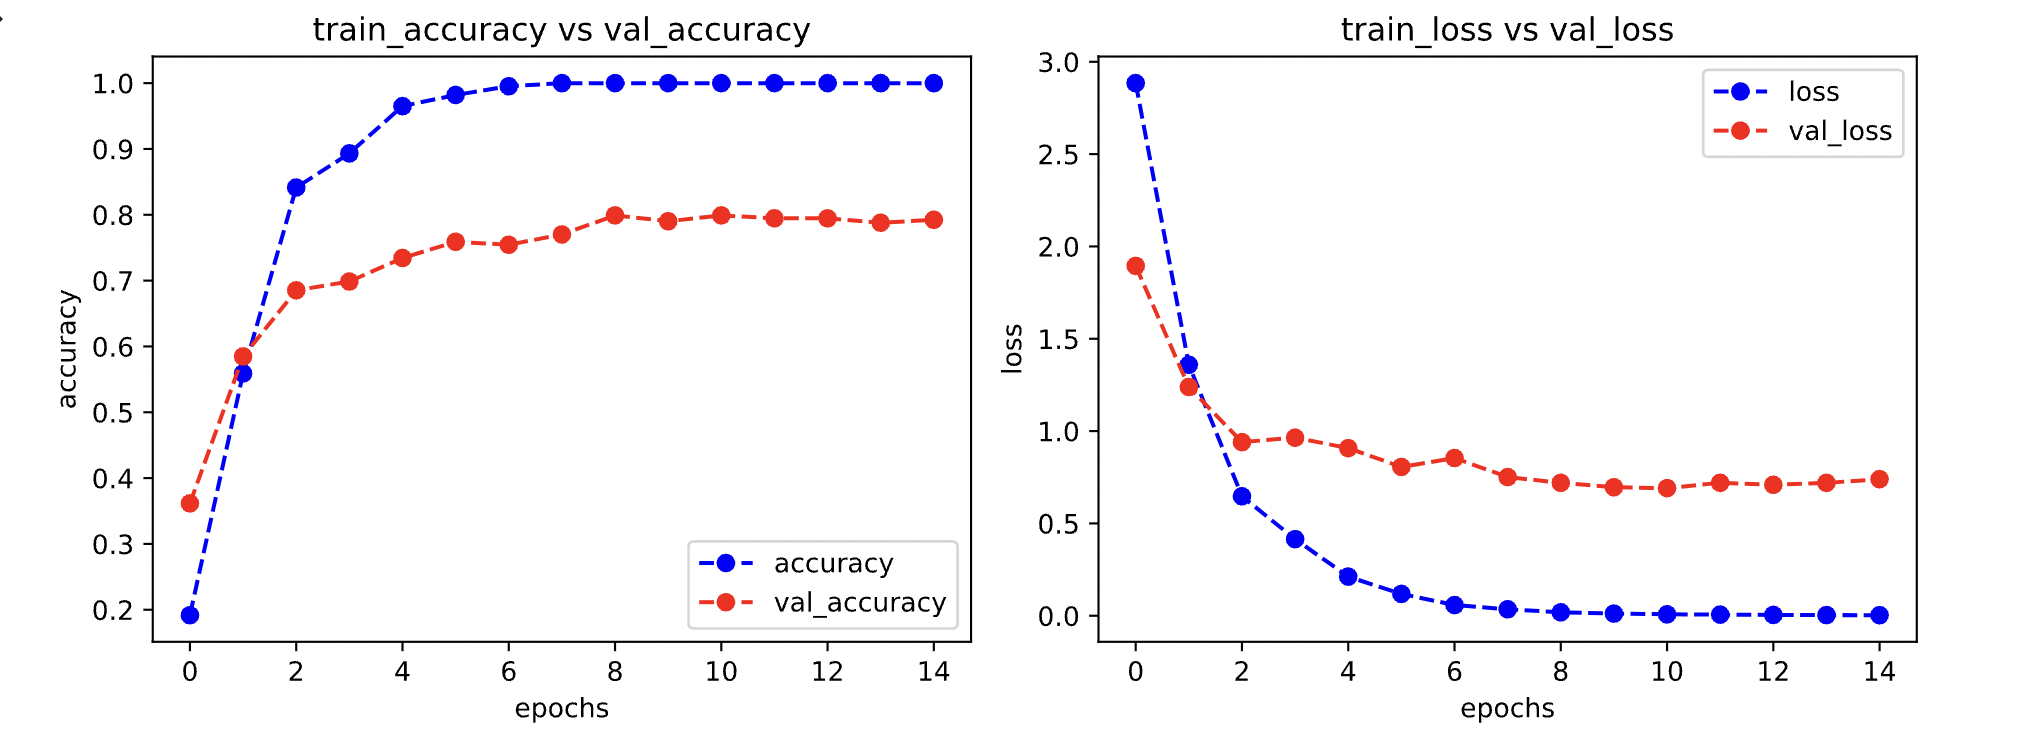
\includegraphics[width=16cm, height=5cm]{./figures/vgg-acc.jpg}
    \caption{Train (Validation) accuracy (loss) changes as number of epochs increases}
    \label{pic:loss-vgg16}
\end{figure}

We summarize the accuracy, weighted average precision and recall rate, and F1-score of the predicted result on the test dataset. The result is quite promising compared with our self-built CNNs. 

\begin{table*}[!htbp]
    \small
	\centering
	\begin{tabularx}{0.6\textwidth}{ccccc}
		\toprule
		\textbf{Support}
       &  \textbf{Accuracy}
        & \textbf{Precision} 
        & \textbf{Recall} 
        & \textbf{F1-Score} \\

        \midrule
        452
        & 80\%
        & 85\%
        & 77\%
        & 81\%\\
		\bottomrule
	\end{tabularx}%
	\label{tab:result2}%
	\caption{Performance indicator on the test set}
\end{table*}%

\paragraph{ResNet Architecture}

ResNet, short for Residual Network\cite{he2016deep}, was proposed in 2015 by researchers at Microsoft Research. ResNet is mainly designed to solve the complex recognition problems. More additional layers are stacked in the deep neural networks, resulting in an improved accuracy and an overall performance.

In order to solve the problem of the vanishing/exploding gradient, ResNet uses skip connections by allowing an alternate shortcut path for the gradient to flow through. The skip connection skips training from a few layers and connects directly to the output. The approach behind this network is that instead of learning the underlying mapping, we allow the network to fit the residual mapping. Hence, instead of letting the network fit the initial mapping $H(x)$, $F(x) := H(x) – x$ will be used which gives $H(x) := F(x) + x$. 
 
The advantage of adding this type of skip connection is that if any layer hurts the performance of architecture, then it will be skipped by regularization. So this results in training an intense neural network without the problems caused by vanishing/exploding gradient. Fig.\ref{pic:resnet} shows the detailed architecture of ResNet:


\begin{figure}[H]
    \centering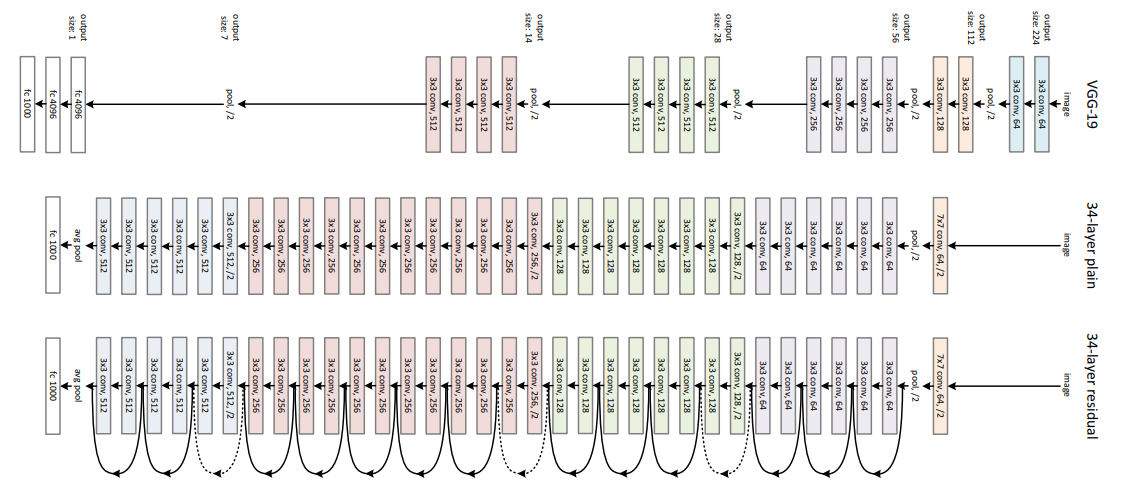
\includegraphics[width=12cm]{./figures/ResNet.png}
    \caption{ResNet-Architecture}
    \label{pic:resnet}
\end{figure}

This network uses a 34-layer plain network architecture inspired by VGG-19 in which then the shortcut connection is added. These shortcut connections then convert the architecture into the residual network. We imported the Keras API to realize the ResNet implementation. 

\begin{lstlisting}[language=python]
from keras.applications.resnet import ResNet50
resnet = ResNet50(include_top=False, weights='imagenet', input_shape=(264,264,3))
for layer in resnet.layers:
    layer.trainable=False
x = Flatten()(resnet.output)
x = Dense(512,activation='relu')(x)
x = Dense(512,activation='relu')(x)
x = Dense(256,activation='relu')(x)
x = Dense(128,activation='relu')(x)
prediction = Dense(13,activation='softmax')(x)
model = Model(inputs=resnet.input, outputs=prediction)
model.compile(optimizer='adam', loss='categorical_crossentropy', metrics=['accuracy'],weighted_metrics=[tf.keras.metrics.Precision(), tf.keras.metrics.Recall()])
history=model.fit_generator(train_data,validation_data=test_data,epochs=150,steps_per_epoch=len(train_data),validation_steps=len(test_data))
\end{lstlisting}
\vspace{-0.6cm}

As seen from the graph below that the ResNet architecture needs much more epochs to converge, while the prediction accuracy rate is not high as before, which means this architecture may not be very suitable for our task. Some possible improvement strategies are using the data augmentation method to enlarge the training dataset and adding more fully connected layers to fine-tune the model.

\begin{figure}[H]
    \begin{minipage}[t]{0.47\textwidth}
        \centering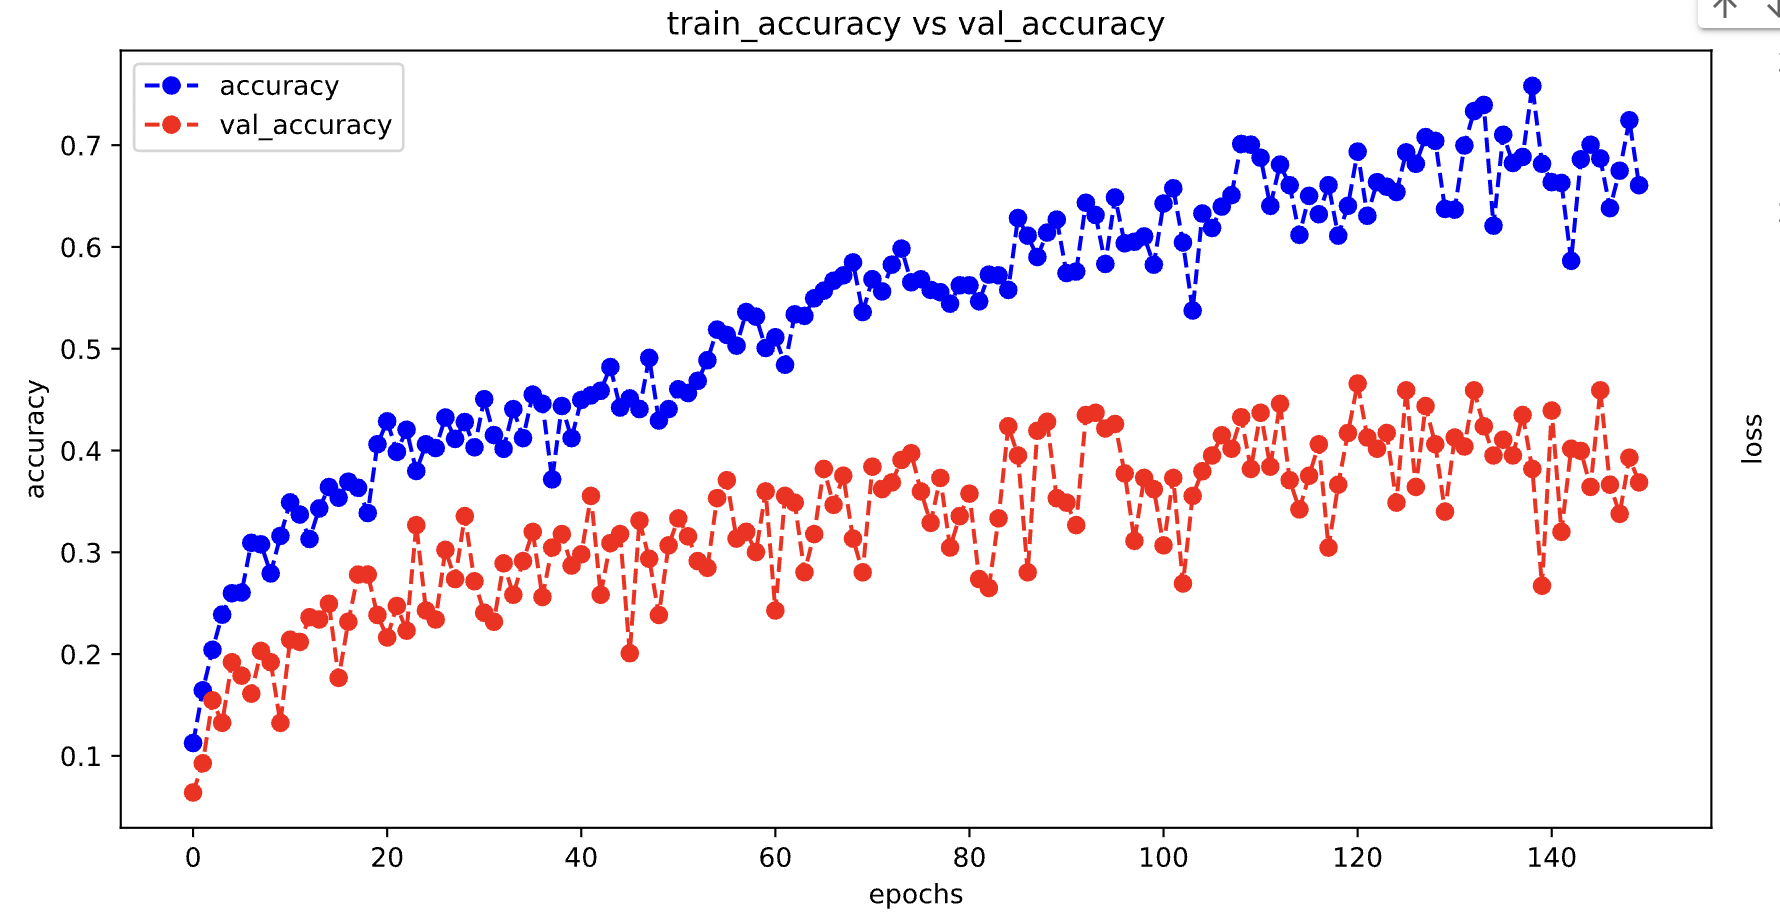
\includegraphics[width=8cm, height=5cm]{./figures/res1.jpg}
        \caption{Train (Validation) accuracy changes}
        \label{pic:correct2}
    \end{minipage}
    \qquad
    \begin{minipage}[t]{0.47\textwidth}
        \centering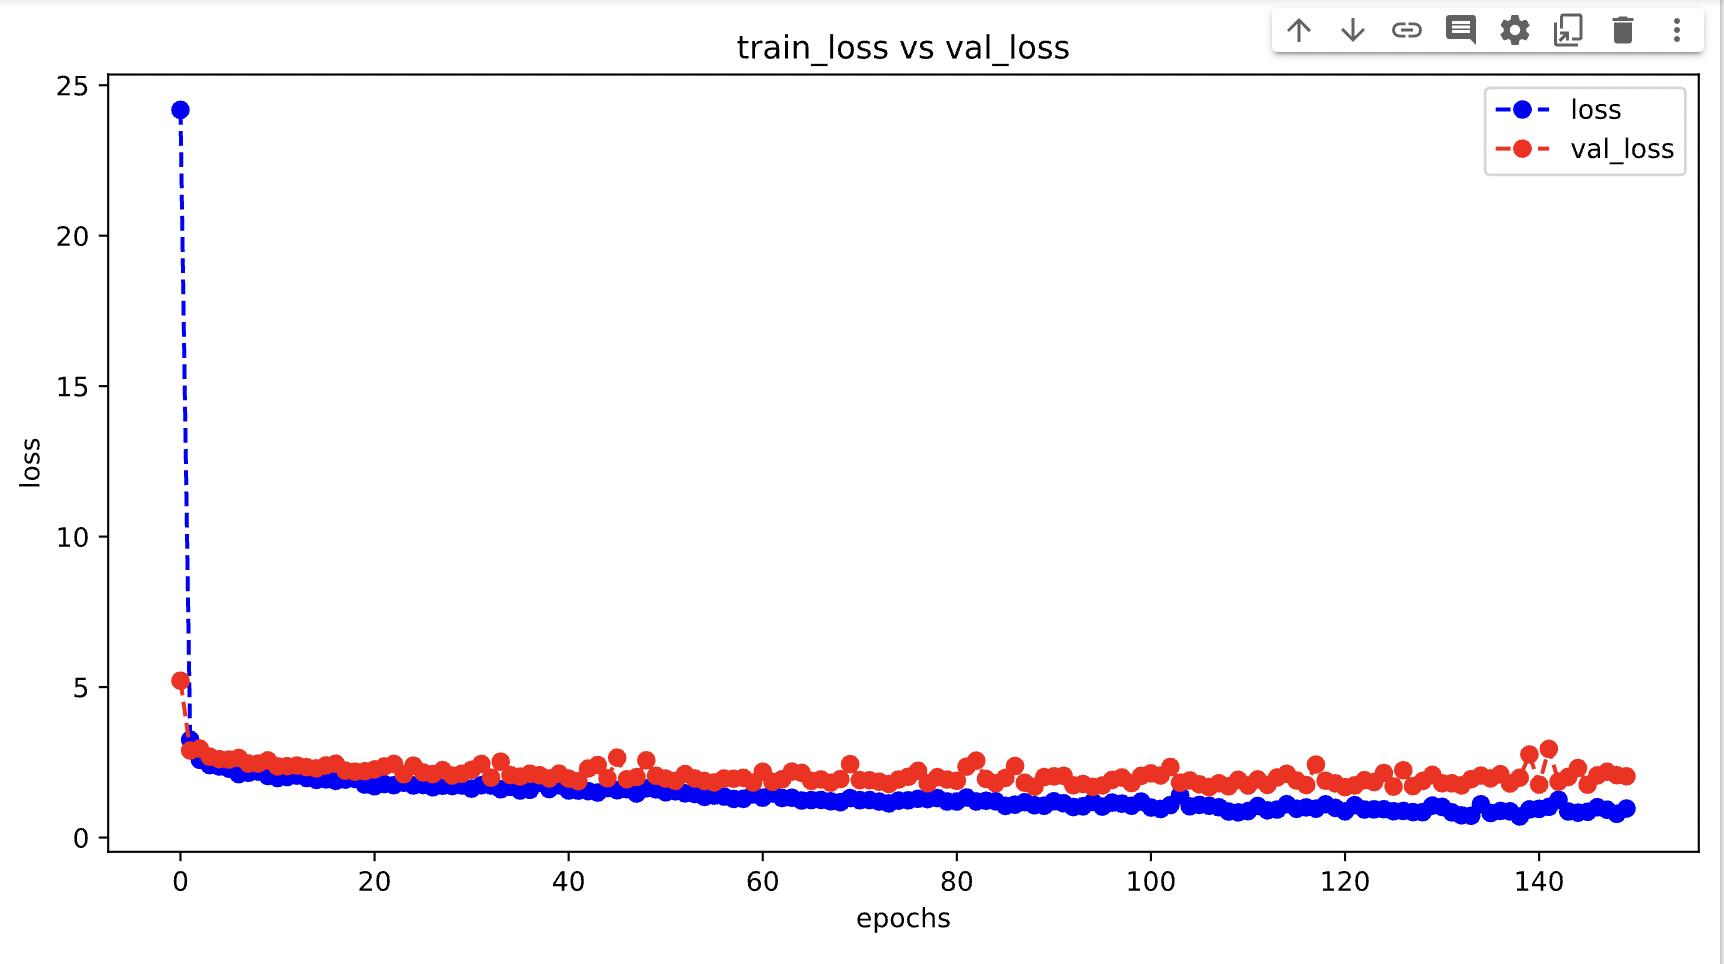
\includegraphics[width=8cm, height=5cm]{./figures/res2.jpg}
        \caption{Train (Validation) loss changes}
        \label{pic:wrong2}
    \end{minipage}
    
\end{figure}

Finally, we summarize the accuracy, weighted average precision and recall rate, and the F1-score of the predicted result on the test dataset.

\begin{table*}[!htbp]
    \small
	\centering
	\begin{tabularx}{0.6\textwidth}{ccccc}
		\toprule
		\textbf{Support}
       &  \textbf{Accuracy}
        & \textbf{Precision} 
        & \textbf{Recall} 
        & \textbf{F1-Score} \\

        \midrule
        452
        & 42\%
        & 40\%
        & 38\%
        & 39\%\\
		\bottomrule
	\end{tabularx}%
	\label{tab:result3}%
	\caption{Performance indicator on the test set}
\end{table*}%

\paragraph{Inception Network Architecture}

Inception network\cite{szegedy2015going} achieved a milestone in CNN classifiers when previous models were just going deeper to improve the performance and accuracy but compromising the computational cost. The Inception network, allows you to maintain a "computational budget" while increasing the depth and width of the network.

The main problems that deeper CNN models like VGGNet face are as follows:
\begin{itemize}
    \item Although previous networks like VGG achieved significant accuracy on ImageNet datasets, the computational cost of deploying these types of models was very high due to their deep architecture.
    \item Very deep networks are prone to overfitting. It is also difficult to pass gradient updates across the network.
\end{itemize}

Here is an intuitive guide to the Inception Network Architectures:

\begin{figure}[H]
    \centering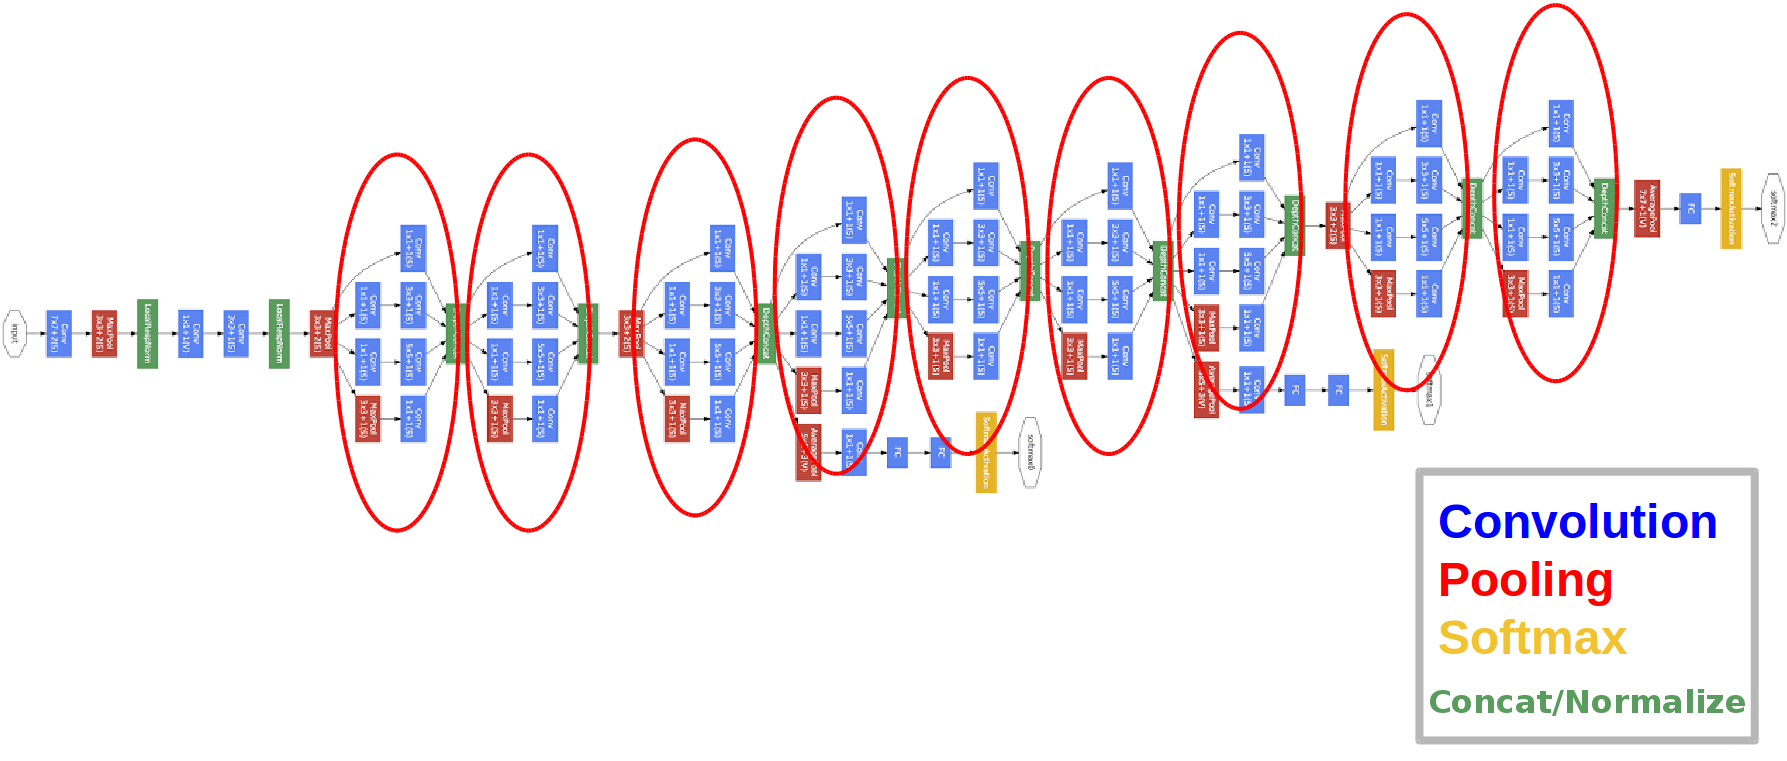
\includegraphics[width=12cm]{./figures/inception.png}
    \caption{Inception Network-Architecture.}
    \label{pic:inception}
\end{figure}

Deep Convolutional Networks are computationally expensive. The inception network can be reduced drastically by introducing the 1 x 1 convolution. We used the pre-trained Inception Network model and fine-tuned several fully connected layers to realize it. 

\begin{lstlisting}[language=python]
from keras.applications.inception_v3 import InceptionV3
inception = InceptionV3(include_top=False, weights='imagenet', input_shape=(264,264,3))
for layer in inception.layers:
    layer.trainable=False
x = Flatten()(inception.output)
x = Dense(512,activation='relu')(x)
x = Dense(256,activation='relu')(x)
x = Dense(128,activation='relu')(x)
x = Dense(64,activation='relu')(x)
prediction = Dense(13,activation='softmax')(x)
model = Model(inputs=inception.input, outputs=prediction)
model.compile(optimizer='adam', loss='categorical_crossentropy', metrics=['accuracy'],weighted_metrics=[tf.keras.metrics.Precision(), tf.keras.metrics.Recall()])
history=model.fit_generator(train_data,validation_data=test_data,epochs=20,steps_per_epoch=len(train_data),validation_steps=len(test_data))
\end{lstlisting}
\vspace{-0.6cm}

It can bee seen that the training accuracy converges rapidly to 1, the validation accuracy stays at roughly 70\% after 4 epochs and then keeps fluctuating.

\begin{figure}[H]
    \centering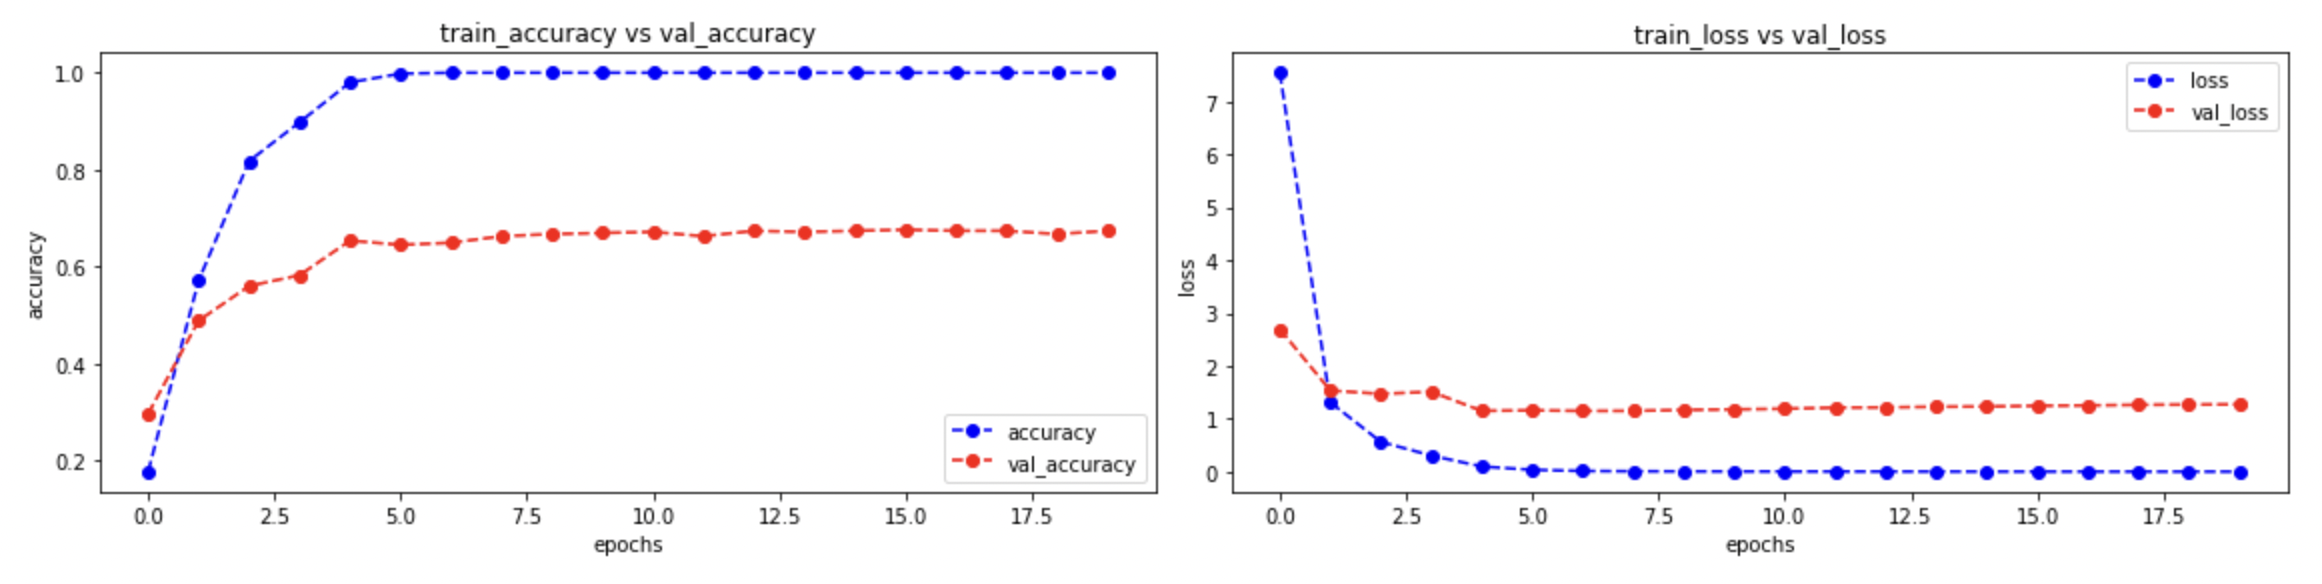
\includegraphics[width=16cm, height=5cm]{./figures/inc-acc.jpg}
    \caption{Train (Validation) accuracy (loss) changes as number of epochs increases}
    \label{pic:vgg16}
\end{figure}

We summarize the accuracy, weighted average precision and recall rate, and the F1-score of the predicted result on the test dataset.

\begin{table*}[!htbp]
    \small
	\centering
	\begin{tabularx}{0.6\textwidth}{ccccc}
		\toprule
		\textbf{Support}
       &  \textbf{Accuracy}
        & \textbf{Precision} 
        & \textbf{Recall} 
        & \textbf{F1-Score} \\

        \midrule
        452
        & 67\%
        & 71\%
        & 65\%
        & 68\%\\
		\bottomrule
	\end{tabularx}%
	\label{tab:result4}%
	\caption{Performance indicator on the test set}
\end{table*}%

\subsubsection{FaceNet}
Finally, we use the powerful FaceNet which is designated to face recognition problems to classify the Bollywood celebrities.
\paragraph{Feature Extraction by FaceNet}
For the feature extraction in this section, we use the FaceNet model \cite{schroff2015facenet}, a deep convolutional neural network trained with a triple loss function that encourages vectors of the same identity to become more similar while vectors of different identities are expected to become less similar. About the underlying strategy of the model, it firstly selects a target image randomly. It then chooses an image of the same person as a positive example and an image of a different person as a negative example. Then, it adjusts the model parameters so that the positive sample is closer to the target than the negative example. The FaceNet model then repeats the same process iteratively until there are no more changes to be done. The detailed architecture is as shown in fig.\ref{pic:facenetX}. 

To get the face embedding, we call the data in ``data\_bw.npz'', and then use FaceNet (similar to PCA) to extract high-quality features from the face and generate face embeddings by compressing the face into a vector of 128 values as shown in fig.\ref{pic:facenet3}. 

\begin{figure}[H]
    \centering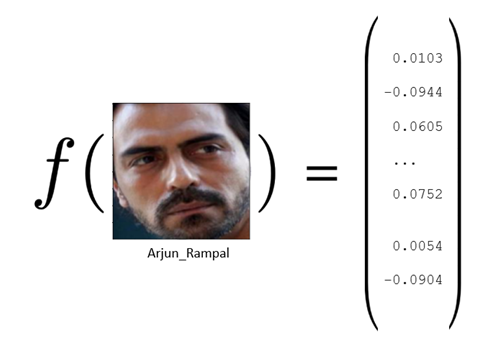
\includegraphics[width=8cm]{./figures/facenet3.png}
    \caption{Face embedding of the face region generated by the first training data of Arjun Rampal}
    \label{pic:facenet3}
\end{figure}

We save this section's final generated face embedding as ``data\_bw-embeddings.npz'' in NumPy ``npz'' format. Suppose we interpret the embeddings as points in a two-dimensional coordinate system and insert six face images of Deepika Padukone and Govinda respectively, the result will be like that in the fig.\ref{pic:facenet4}, where the embeddings of the same person's face is closer. As for the meaning contained in the values in the embedded vector, it is as difficult to explain as PCA. 

\begin{figure}[H]
    \centering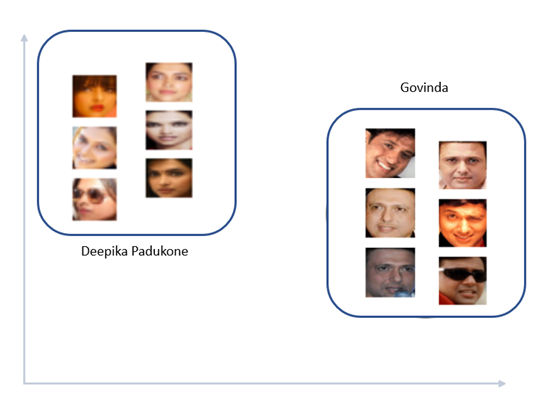
\includegraphics[width=8cm]{./figures/facenet4.png}
    \caption{Face images plotted in 2D cartesian coordinate}
    \label{pic:facenet4}
\end{figure}


\paragraph{Classification by SVM/MLP}
After obtaining face embeddings, we use support vector machines and multi-layer perceptrons for classification, respectively, to answer ``who is this person''. For MLP, it includes every layer starting from the Flatten() layer in 3.2.1.1.

From the table below, we found that SVM without parameter tuning can achieve an accuracy of 98.01\%. In order to further improve the classification accuracy, we tried the random search method for the hyper-parameter of SVM, and 0.23\% increased the accuracy. Also, we tried to do the classification problem by the fully connected neural network MLP. It turns out that the performance of MLP is roughly the same as that of SVM after hyperparameter tuning (denoted as SVM*) in terms of accuracy and recall. However, the precision and F1-Score indicate that SVM* is slightly better than MLP.

\begin{table*}[!htbp]
    \small
	\centering
	\begin{tabularx}{0.7\textwidth}{cccccc}
		\toprule
		\textbf{Method} & \textbf{Support}
       &  \textbf{Accuracy}
        & \textbf{Precision} 
        & \textbf{Recall} 
        & \textbf{F1-Score} \\

        \midrule
        SVM & 452& 98.01\% & 98.13\% & 98.01\% & 98.02\%\\
        SVM* & 452& 98.23\% & 98.35\% & 98.23\% & 98.24\%\\
        MLP & 452& 98.23\% & 98.32\% & 98.23\% & 98.23\%\\
        
        
		\bottomrule
	\end{tabularx}%
	\label{tab:result3}%
	\caption{ Performance indicator on the test set}
\end{table*}%


\begin{figure}[H]
    \begin{minipage}[t]{0.49\textwidth}
        \centering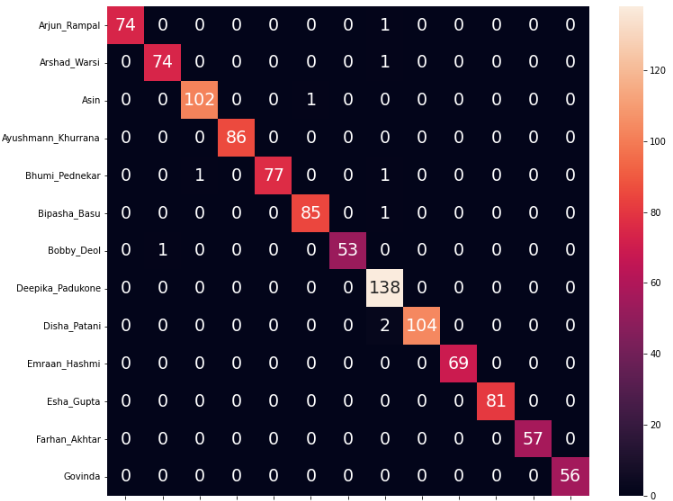
\includegraphics[width=7.2cm]{./figures/svm_star_confusion_train.png}
        \caption{SVM* confusion matrix on the training set}
        \label{pic:confusion3}
    \end{minipage}
    \qquad
    \begin{minipage}[t]{0.49\textwidth}
        \centering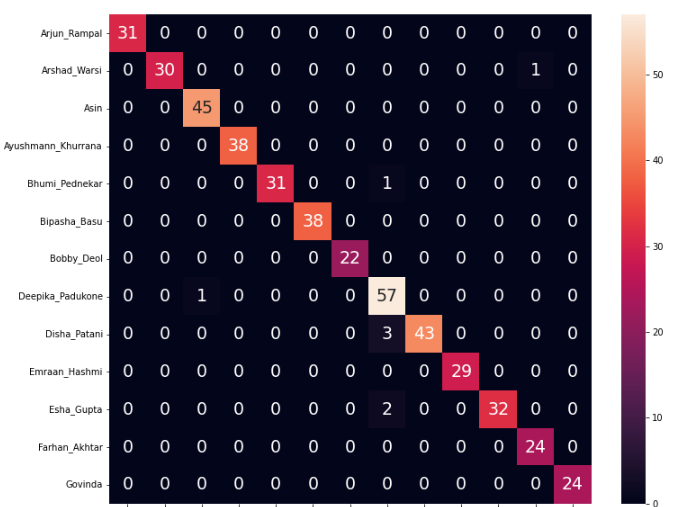
\includegraphics[width=7.2cm]{./figures/svm_star_confusion_test.png}
        \caption{SVM* Confusion matrix on the test set}
        \label{pic:confusion4}
    \end{minipage}
\end{figure}

We can also make some inferences on the reasons for the high accuracy. The first guess is that the stars we selected are not similar in appearance and their embeddings are therefore better distinguishable. And the second is that our dataset is a star image dataset. A star will likely take multiple photos at the same event, which means the makeup and the shooting environment are also the same, so the randomly generated training set and test set are likely to include photos from the same event and thus leads to a good classification result. Hence, although our dataset produces good results, it may not be ideal in real-life applications, such as mobile phone face unlocking. Sometimes it may not be possible to distinguish a pair of sisters with similar looks, and sometimes it cannot identify users with no makeup if only the image after makeup is used as training data.



\section{Discussion}
\subsection{Performance Summary}
By summarizing the training performance above, we reach the following performance table \ref{comparison}. The results show that after the feature extraction by FaceNet, both SVM and MLP performs much better than all the previous CNN models, achieving over 98\% of the test accuracy, precision, recall, and the F1-score. The triplet loss mechanism in FaceNet and the pre-trained weights from a much larger dataset prove extremely effective to apply on the celebrity recognition problem.
\begin{center}
    \small
    \resizebox*{0.65\textwidth}{4cm}{
    \begin{tabular}{|l|cccc|}
    \hline
    \diagbox{Model}{Metric}
    & Accuracy   & Precision & Recall & F1-Score\\
    \hline
    CNN1   &  51\% & 49\% & 52\% & 50\% \\
    CNN2   &  60\% & 65\% & 57\% & 59\% \\
    AlexNet   &  62\% & 63\% & 62\% & 62\% \\
    VGG16   &  80\% & 85\% & 77\% & 81\% \\
    ResNet  &  42\% & 40\% & 38\% & 39\% \\
    Inception Network   &  67\% & 71\% & 65\% & 68\% \\
    FaceNet+SVM   &  98\% & 98\% & 98\% & 98\% \\
    FaceNet+MLP  &  98\% & 98\% & 98\% & 98\% \\

    \hline
    \end{tabular}}
    \fcaption{performance comparison}
    \label{comparison}
\end{center}

\subsection{Improvements and Applications}
One of the further improvements is to consider the one-shot learning problem. One-shot learning \cite{fei2006one} is a classification task where only one example is given for each class to train the model, which means a person needs to be recognized using just one single image. For instance, facial recognition technology is used at airports and border crossings to determine whether the person standing in front of the machine is the same as the photo on the passport during passport control. 

We can calculate the triplet loss (and it is also the crucial part of the FaceNet architecture) to solve the one-shot learning problem. The triplet loss trains the neural network by giving it three images: an anchor image, a positive image, and a negative image. The neural network must adjust its parameters so that the feature encoding values for the anchor and positive image are very close while that of the negative image is very different. FaceNet outperforms all other models in this project since it uses the triplet loss mechanism to relieve the shortage of training data. 

In real life, face recognition technology has many other application scenarios, including the use of face detection and comparison function for identity verification, electronic attendance of employees for enterprises, security monitoring, etc. Face search service can also retrieve the library and input face most similar N face picture and similarity, and according to the time, place and behavior information of the returned picture, to assist customers in achieving trajectory analysis.

\section{Conclusion}
Face detection is always a complicated task that scholars work on for decades to strive for a good predictor. In this celebrity recognition project, we use different models and compare their predicting performance on the test dataset. We first use the Multi-task Cascaded Convolutional Networks to detect the location of faces. Two self-built CNNs are used to extract the information and predict the dataset. Then classical CNNs in the literature are applied to compare the performance. Finally, the renowned FaceNet is built to further extract the features, and then both SVM and MLP are used to give the predictions. 

The results show that after the feature extraction by FaceNet, both SVM and MLP performs much better than all the previous CNN models, achieving over 98\% of the test accuracy, precision, recall, and the F1-score. The triplet loss mechanism in FaceNet and the pre-trained weights from a much larger dataset prove extremely effective to apply on the new celebrity recognition problem.



\newpage

\bibliographystyle{plain}
\bibliography{custom}

\end{document}








% \begin{lstlisting}[language=R]
% set.seed(1)
% # Standardization
% x = scale(train[,-ncol(train)], center = T, scale = T)
% dat = data.frame(x = x, y = as.factor(Class))
% # first tuning
% tune.out = tune(svm, y ~ ., data = dat, kernel = "radial", 
%                 ranges = list(cost = seq(1,600,100),
%                 gamma  = seq(0.5, 3, 0.5)))
% # second tuning
% tune.out = tune(svm, y ~ ., data = dat, kernel = "radial", 
%                 ranges = list(cost = seq(0.1, 10, 2),
%                 gamma  = seq(0.2, 0.8, 0.1)))
% # third tuning
% tune.out = tune(svm, y ~ ., data = dat, kernel = "radial", 
%                 ranges = list(cost = seq(5, 8, 1),
%                 gamma  = seq(0.01, 0.3, 0.05)))
% \end{lstlisting}
% \vspace{-0.6cm}


% \begin{center}
%     % \small
%     \begin{tabular}{|c | c|}
%     \hline
%     Model   &  Best Performance \\
%     \hline
%     Logistic Regression   &  92.26\% \\
%     \hline
%     LDA   &  89.77\% \\
%     \hline
%     Naive Bayes   &  90.31\% \\
%     \hline
%     QDA   &  91.08\% \\
%     \hline
%     K-Nearest Neighbors  &  92.12\%\\
%     \hline
%     Classification Tree  &  86.97\%\\
%     \hline
%     Random Forest   &  92.56\% \\
%     \hline
%     Boosting   &  92.67\% \\
%     \hline
%     SVM (linear kernel) & 92.74\% \\
%     \hline
%     SVM (polynomial kernel) & 92.90\% \\
%     \hline
%     SVM (radial kernel) & \textbf{93.28\%} \\
%     \hline

%     \hline
%     \end{tabular}
%     \fcaption{Model comparison results}
%     \label{Model comparing results}
% \end{center}


% \begin{table*}[!htbp]
%     \small
% 	\centering
% 	\begin{tabularx}{1\textwidth}{cccccccc}
% 		\toprule
%         \textbf{BARBUNYA}
%         & \textbf{BOMBAY} 
%         & \textbf{CALI} 
%         & \textbf{DERMASON} 
%         & \textbf{HOROZ}
%         & \textbf{SEKER}
%         & \textbf{SIRA}
%         & \textbf{Overall}\\

%         \midrule
%         0.9182
%         & 1.0000
%         & 0.9459
%         & 0.9345
%         & 0.9606 
%         & 0.9308
%         & 0.8938
%         & \textbf{0.9321}\\
% 		\bottomrule
% 	\end{tabularx}%
% 	\label{tab:addlabel}%
% 	\caption{Accuracy on each separate class}
% \end{table*}%



% \begin{algorithm2e}[H]
%     \caption{\textbf{Best subset selection for multinomial logistic model}}    
%     \label{alg:bs selection}
%     \lnlset{alg:gm-1}{1}{Initialization: let $M_0$ be the null model, which contains no predictors.}\\
%     % \lnlset{alg:gm-1}{1}{Initialization: ~~Select an initial point  $x^0 \in \Rn$ and parameter $\gamma, \gamma_1, \gamma_2, \sigma \in (0,1)$ and \texttt{tol}.} \\ 
%     \For{$k = 0,1,... p,$}{
%     \lnlset{alg:gm-2}{2}{Fit all $C_p^k$ logistic models that contain exactly k predictors, i.e., selecting the 7-th class as the baseline, then for all $s=1,2,\dots ,6:$
%     %
%     \[ Pr(Y=s|X=x)=\frac{e^{\beta_{s0}+\beta_{s1}x_1+\dots + \beta_{sk}x_k}}{1+\sum_{l=1}^{6}e^{\beta_{l0}+\beta_{l1}x_1+\dots + \beta_{lk}x_k}} \]} \\
%     %
%     \lnlset{alg:gm-3}{3}{Pick the best among these $C_p^k$ logistic models, and denote it as $M_k$. Here \texttt{best} is defined as having the smallest \textbf{deviance:} $D(y;\hat{\mu})=-2log(l_0/l_S)$.} \\
%     } 
%     \lnlset{alg:gm-4}{4}{Select a single best model from among $M_0,\dots,M_p$ using cross-validated overall error rate, or $C_p$ (AIC) and BIC for classification.} \\
%     \end{algorithm2e}

% One can also considered adding interaction terms to the model to increase the complexity and accuracy. Models of different parameters can be compared using criteria including AIC and BIC.




